\documentclass[11pt,a4paper]{article}
\usepackage[T1]{fontenc}
\usepackage[utf8]{inputenc}
\usepackage{mathptmx}
\usepackage[scaled=0.92]{helvet}
\usepackage[margin=1in]{geometry}
\usepackage{amsmath,amssymb}
\usepackage{graphicx}
\usepackage{booktabs,longtable,array,multirow,tabularx,threeparttable}
\usepackage[font=small,labelfont=bf,skip=4pt]{caption}
\usepackage[authoryear,round]{natbib}
\usepackage{xcolor}
\usepackage[colorlinks=true,linkcolor={blue!50!black},citecolor={blue!50!black},urlcolor={blue!50!black}]{hyperref}
\usepackage{microtype}
\usepackage{enumitem}
\usepackage{fancyhdr}
\usepackage{placeins}
\usepackage{flafter}
\renewcommand{\topfraction}{0.9}
\renewcommand{\bottomfraction}{0.8}
\renewcommand{\textfraction}{0.07}
\renewcommand{\floatpagefraction}{0.85}
\setcounter{topnumber}{3}
\setcounter{bottomnumber}{2}
\setcounter{totalnumber}{5}
\setlength{\floatsep}{10pt plus 2pt minus 2pt}
\setlength{\textfloatsep}{10pt plus 2pt minus 2pt}
\setlength{\intextsep}{8pt plus 2pt minus 2pt}
\raggedbottom
\setlist{itemsep=2pt,topsep=3pt}
\setlength{\parskip}{3pt}
\renewcommand{\arraystretch}{1.12}
\graphicspath{{figures/}}
\pagestyle{fancy}
\fancyhf{}
\fancyhead[L]{\small Zero-Days at Machine Speed}
\fancyhead[R]{\small Chongmankhong (2026)}
\fancyfoot[C]{\thepage}
\renewcommand{\headrulewidth}{0.4pt}

\title{\textbf{Zero-Days at Machine Speed:\\ AI-Driven Vulnerability Discovery, Systemic Cyber Risk\\ in Banking, and Implications for Central Banks}\\[4pt]
\large Evidence from 405,375 CVE Records and the CISA KEV Catalogue, with Scenarios for Thailand}
\author{Thanatchon Chongmankhong}
\date{Preprint --- 12 November 2026}

\begin{document}
\maketitle
\thispagestyle{empty}

\begin{abstract}
\noindent
Artificial intelligence (AI) systems now find software vulnerabilities at industrial scale. We ask what this means for banks, payment systems and central banks, with a focus on Thailand. We assemble four bodies of evidence: the full CVE List V5 (405,375 published records, snapshot of 12 November 2026); the CISA Known Exploited Vulnerabilities (KEV) catalogue (1,779 entries); a curated set of 33 financial-sector cyber incidents (2011--2025) and 11 hardware trust-anchor cases; and a group-level framework for the Thai financial system. We find, first, a \emph{disclosure shock}: CVE publications in January--October 2026 were 2.27 times the 2025 level, and monthly volume quadrupled between October 2025 and October 2026, led by large commercial vendors (Google Chrome $\times$33, Oracle $\times$13, Microsoft $\times$4). Second, at least 1,598 CVEs credit an AI model, agent or AI-native organisation; the monthly count has doubled roughly every four months since mid-2025, and AI-credited vulnerabilities are as severe as human-credited ones (mean CVSS 6.93 vs.\ 6.98, $p=0.66$). This is a lower bound, because vendors that publish most commercial CVEs record no credits. Third, exploitation has risen more slowly than discovery: KEV additions reached 295 in 2026 to date (245 in 2025), but the share of new CVEs exploited within 180 days fell from 3.9 to 2.6 per 1,000. A KEV-based zero-day proxy reproduces published industry counts for 2022--2024 within 7\%. Only 15 AI-credited CVEs have entered KEV, almost all as n-days found by offensive-security firms. Fourth, the incident record shows that zero-days reach financial institutions through shared commercial products---file-transfer appliances, mail servers and perimeter devices---not through core banking systems; perimeter devices rose from 14.6\% to 21.0\% of KEV additions between 2022 and 2026. A stylised Monte Carlo model of a Thai-like system, calibrated to KEV event rates, shows that a threefold AI-driven increase in offensive capacity raises the annual probability of a systemic payment disruption about fivefold (4.0--6.8$\times$ across parameterisations), that AI-enabled defence removes 50--75\% of that increase, and that vendor concentration amplifies it by a further 36--64\%. We draw ten implications for central banks, including patch-latency supervision of internet-facing products, a sector-wide register of shared-vendor concentration, and pooled AI-enabled defensive capacity.

\medskip
\noindent\textbf{Keywords:} zero-day vulnerabilities; artificial intelligence; cyber risk; financial stability; central banking; payment systems; Thailand\\
\noindent\textbf{JEL:} E58, G21, G28, O33\quad \textbf{arXiv:} cs.CR (cross-list cs.AI, q-fin.RM)
\end{abstract}

\vspace{4pt}
\noindent\fbox{\parbox{0.97\textwidth}{\small\textbf{Scope and ethics.} This study uses only public data. It contains no exploit code, no proof-of-concept, no scanning or testing of any institution's systems, and no statement about the security of any named Thai institution. The Thai analysis is at the level of institution groups and is based on structured expert judgement. Case descriptions and industry benchmark figures were coded from public reporting and should be verified against primary sources before citation.}}

\newpage
\tableofcontents
\newpage

%=====================================================================
\section{Introduction}\label{sec:intro}

For most of the history of computing, finding a previously unknown and exploitable software vulnerability---a \emph{zero-day}---was slow, expensive and the preserve of a small community of specialists. That scarcity shaped who could attack critical systems. The best-known example, Stuxnet, used four Windows zero-days and stolen code-signing certificates to sabotage uranium-enrichment centrifuges at Iran's Natanz facility \citep{falliere2011stuxnet,langner2013kill,zetter2014countdown}; it required resources available only to states. Banks have historically been attacked by cheaper means: stolen credentials, phishing, insiders and known but unpatched vulnerabilities.

Since 2024 that scarcity has eroded. Large language model (LLM) agents have moved from solving capture-the-flag exercises \citep{zhang2024cybench} to exploiting known web vulnerabilities from their advisories \citep{fang2024oneday,zhu2024teams} and to finding new, real vulnerabilities in widely deployed software \citep{bigsleep2024,darpa2025aixcc}. Frontier AI developers now operate dedicated vulnerability-research agents \citep{openai2025aardvark,deepmind2025codemender,anthropic2026glasswing}, and at least one threat report describes an espionage campaign in which an AI agent executed most tactical steps \citep{anthropic2025espionage}. If the cost of discovering zero-days falls by an order of magnitude, the threat model for the financial system changes.

This paper asks six questions:
\begin{enumerate}[label=\textbf{RQ\arabic*.},leftmargin=3.2em]
\item How much vulnerability discovery is now done with AI, by whom, and with what trajectory?
\item Which commercial software has been exploited as a zero-day, and how has exploitation changed?
\item Are hardware-wallet zero-days relevant to banks?
\item Where is the global banking system exposed, and would AI-discovered zero-days be used against it?
\item In Thailand, which groups of institutions are likely targets and which are most vulnerable?
\item Should central banks, including the Bank of Thailand (BOT), treat this as a priority, and what should they do?
\end{enumerate}

We answer with four bodies of evidence. The first is the complete CVE List V5 \citep{cveprogram2026}, from whose free-text credits we identify AI-credited discoveries using a transparent, auditable lexicon. The second is the CISA KEV catalogue \citep{cisa2026kev}, which we turn into a panel of exploited vulnerabilities with product categories, disclosure-to-listing lags and a validated zero-day proxy. The third is a curated set of financial-sector incidents and hardware trust-anchor cases. The fourth is a group-level framework for Thailand together with a Monte Carlo model of shared-vendor contagion calibrated to KEV event rates.

\paragraph{Contributions.} (i) We provide what is, to our knowledge, the first census of AI-credited CVEs across the full CVE corpus, with a documented lexicon and its known false positives. (ii) We document a 2026 disclosure shock in commercial software and show that exploitation has grown more slowly than disclosure. (iii) We validate a simple KEV-based zero-day proxy against published industry counts. (iv) We connect vulnerability data to financial-sector exposure through a bank-weighted exploitation-pressure measure and an incident record. (v) We offer a reproducible scenario model and a ten-point policy agenda for central banks. All code and derived data accompany the paper.

\paragraph{Headline findings.} AI-assisted discovery is real, fast-growing and so far mostly defensive; exploitation of commercial perimeter and IT-management products is the main channel through which zero-days reach financial institutions; and the main systemic risk for a system such as Thailand's is correlated exposure through shared vendors and service providers rather than a direct attack on the core payment infrastructure. Section~\ref{sec:policy} sets out why these findings justify central-bank attention now.

\paragraph{Roadmap.} Section~\ref{sec:background} sets out concepts; Section~\ref{sec:related} reviews related work; Section~\ref{sec:data} describes data and methods. Sections~\ref{sec:shock}--\ref{sec:exposure} present results on disclosure, AI discovery, exploitation, hardware and financial exposure. Section~\ref{sec:thailand} analyses Thailand, Section~\ref{sec:sim} reports the simulation, Section~\ref{sec:policy} discusses policy, and Section~\ref{sec:limits} states limitations.

%=====================================================================
\section{Background and concepts}\label{sec:background}

\subsection{Zero-days, n-days and the exploitation window}
A \emph{zero-day} is a vulnerability exploited before the vendor has disclosed it or made a fix available; an \emph{n-day} is exploited after disclosure, during the period in which users have not yet applied the fix. Figure~\ref{fig:lifecycle} places both on a single timeline. The zero-day window runs from first exploitation to disclosure; the n-day window runs from disclosure until each user deploys the patch. Historical studies found that zero-day attacks often persisted for months before discovery \citep{bilge2012before} and that stockpiled exploits had long expected lifetimes \citep{ablon2017zero}. More recent industry reporting suggests that the time from disclosure to exploitation has collapsed to days \citep{mandiant2024tte}.

\begin{figure}[!htbp]
\centering
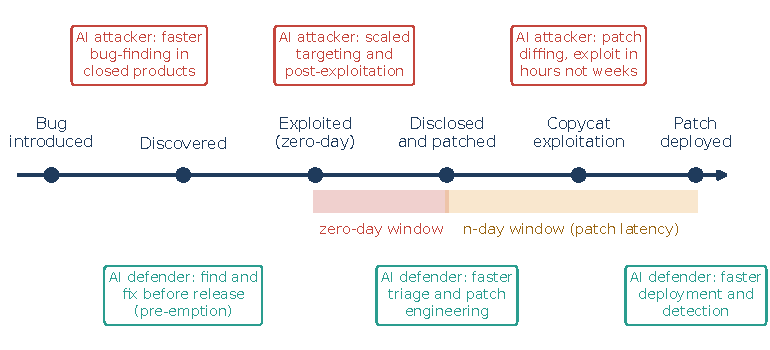
\includegraphics[width=\textwidth]{fig01_lifecycle.pdf}
\caption{Vulnerability lifecycle and points at which AI changes attacker and defender capabilities. Red boxes: offensive uses; green boxes: defensive uses. The zero-day window ends at disclosure; the n-day window ends when each institution deploys the patch.}
\label{fig:lifecycle}
\end{figure}

\subsection{Levels of AI involvement}
We distinguish five levels, because public debate often conflates them:
\begin{description}[leftmargin=1.2em,style=nextline]
\item[L0 --- No AI.] Human researchers using conventional tools such as fuzzers and static analysers.
\item[L1 --- AI-assisted.] Humans use AI for code reading, triage or tooling. This is largely invisible in public records.
\item[L2 --- AI-credited discovery.] An AI system, or an organisation whose product is AI-driven discovery, is credited in the vulnerability record. This is the level we measure.
\item[L3 --- Autonomous discovery and exploitation.] An agent finds and weaponises a vulnerability end-to-end, as demonstrated in competitions and laboratory studies \citep{darpa2016cgc,darpa2025aixcc,zhu2024teams}.
\item[L4 --- AI-orchestrated campaigns.] An agent executes most steps of an intrusion campaign against real targets; at least one such case has been publicly reported \citep{anthropic2025espionage}.
\end{description}
Public data observe L2 directly, L4 occasionally through threat reports, and L1 and L3 hardly at all. Our measurements are therefore lower bounds on AI involvement.

\subsection{Why banks are exposed}
Banks run the same commercial products as other large organisations. These include perimeter VPN and firewall appliances, managed file transfer (MFT), mail and collaboration servers, IT-management and remote-access tools, hypervisors, and enterprise applications. Banks also connect to shared infrastructures: real-time gross settlement (RTGS), retail payment switches, card networks, messaging networks and a small number of IT and cloud providers. A zero-day in a widely used product therefore produces \emph{correlated} exposure across institutions, which is the mechanism through which an operational event becomes a financial-stability event \citep{kashyap2019principles,eisenbach2022cyber,adelmann2020cyber}.

%=====================================================================
\section{Related literature}\label{sec:related}

\paragraph{Vulnerability lifecycle and economics.} Empirical work has measured vulnerability disclosure and patching \citep{frei2006large,arora2010empirical}, the hidden lifetime of zero-days \citep{bilge2012before}, and the economics of exploit stockpiles \citep{ablon2017zero}. Exploitation-prediction models such as EPSS \citep{jacobs2021epss} and catalogues of known-exploited vulnerabilities \citep{cisa2021bod} reflect a shift from severity-based to evidence-based prioritisation. Annual reviews by Google Project Zero, Google's Threat Intelligence Group and Mandiant count in-the-wild zero-days \citep{stone2022review,mandiant2023zeroday,google2024zeroday,gtig2025zeroday} and document a concentration of exploitation on enterprise and perimeter products.

\paragraph{AI offensive and defensive capability.} Benchmarks measure LLM capability on security tasks \citep{bhatt2023purple,zhang2024cybench,zhu2025cvebench}. Agent studies show exploitation of one-day \citep{fang2024oneday} and, with coordinated agent teams, zero-day web vulnerabilities \citep{zhu2024teams}. On the defensive side, Google's Big Sleep reported an exploitable SQLite bug before release \citep{bigsleep2024}. DARPA's AI Cyber Challenge showed cyber-reasoning systems finding and patching real open-source bugs \citep{darpa2025aixcc}, and AI developers have launched agentic security researchers \citep{openai2025aardvark,deepmind2025codemender} and restricted-access defensive programmes \citep{anthropic2026glasswing}. Threat-intelligence reports document misuse, ranging from reconnaissance and scripting \citep{microsoft2024threat} to largely autonomous intrusion operations \citep{anthropic2025espionage}. Most of this work measures capability in controlled settings; we add population-level evidence from the CVE corpus.

\paragraph{Cyber risk and financial stability.} A macro-financial literature models how cyber events propagate: through payment-system impairment \citep{eisenbach2022cyber}, runs \citep{duffie2019cyber}, common exposures and concentration \citep{kashyap2019principles,healey2018future}, and loss distributions \citep{bouveret2018cyber,aldasoro2022drivers}. The IMF identified cyber risk as a growing macro-financial concern \citep{imf2024gfsr,adelmann2020cyber}. Standard setters have issued guidance on financial market infrastructure (FMI) resilience \citep{cpmi2016guidance}, a common lexicon \citep{fsb2018lexicon} and incident-reporting convergence \citep{fsb2023reporting,fsb2025fire}. Supervisors have run cyber stress tests \citep{ecb2024stress} and introduced oversight of critical third parties \citep{eu2022dora,boe2024ctp}. This literature rarely uses vulnerability-level data; we connect the two.

\paragraph{Hardware security.} Research on payment cards \citep{murdoch2010chip,basin2021emv}, secure elements \citep{nemec2017roca,roche2024eucleak}, TPMs \citep{moghimi2020tpmfail}, HSMs \citep{campana2019hsm} and hardware wallets \citep{datko2018walletfail,kraken2020trezor} supplies the material for our discussion of hardware trust anchors.

%=====================================================================
\section{Data and methods}\label{sec:data}

\subsection{CVE List V5}
We downloaded the official bulk release of the CVE List V5 \citep{cveprogram2026} as of 12 November 2026 (425,189 files; 405,375 records in \texttt{PUBLISHED} state). For each record we extract dates, the assigning CVE Numbering Authority (CNA), the first affected vendor and product, the first CWE, the maximum CVSS base score across containers, the CISA ADP SSVC ``Exploitation'' field, and the free-text \texttt{credits}. Only 43.4\% of records published in 2026 carry any credit. Several of the largest commercial CNAs---Microsoft, Google Chrome, Apple, Oracle, SAP, Fortinet and the Linux kernel CNA---recorded none (Table~\ref{tab:vendor}).

\subsection{Identifying AI-credited discoveries}
We apply a lexicon of case-insensitive regular expressions to the credit text (Appendix Table~\ref{tab:lexicon}). \textbf{Tier~1} records name an AI model, agent or tool as finder or co-finder (for example ``Google Big Sleep'', ``XBOW'', ``Claude Security'', ``OpenAI Codex Security'', ``Fluid Attacks' AI SAST Scanner''). \textbf{Tier~2} records credit an AI-native security organisation or an AI laboratory without naming a model (for example AISLE, depthfirst, ZeroPath, Horizon3.ai, or ``OpenAI'' as an organisation). We reviewed random samples of matches for every pattern. This review led to three exclusions: a human researcher whose given name is Claude, a username containing ``gpt'', and the brand name of an established human bug-bounty programme whose name contains the letters ``AI'' (76 false matches before exclusion). Tier~2 is a proxy: AI tooling is likely but not certain for each record. Because credit coverage is incomplete and AI assistance at level L1 is rarely credited, all counts are lower bounds. We also classify the affected software into domains with keyword rules on vendor, product and CNA.

\subsection{KEV exploitation panel}
The KEV catalogue \citep{cisa2026kev} lists vulnerabilities with reliable evidence of in-the-wild exploitation. We map each entry to one of 15 product categories with ordered keyword rules (Appendix~\ref{app:rules}); 7.1\% remain unclassified. We merge the CVE publication date and compute the listing lag
\begin{equation}
\ell_i = d^{\text{KEV}}_i - d^{\text{pub}}_i \quad\text{(days)}.
\end{equation}
The catalogue opened on 3 November 2021 with a back-filled list, so we use lags only for CVEs published on or after that date ($n=898$).

\paragraph{Zero-day proxy.} We call an entry \emph{early-listed} if $\ell_i \le 7$. A vulnerability that is already exploited when it is disclosed is typically listed within days, whereas n-days are listed after weeks or months. We benchmark annual counts of early-listed vulnerabilities against published industry counts of in-the-wild zero-days (Section~\ref{sec:exploitation}).

\paragraph{Right-censoring.} Recent CVEs have had less time to be exploited and listed. For trend comparisons we therefore use a censoring-robust cohort: CVEs published from 2022 up to 180 days before the snapshot, counting only listings within 180 days of publication.

\subsection{Bank-weighted exploitation pressure}
Not every product category matters equally to banks. We assign a banking-relevance weight $w_c\in[0,1]$ to each category (Appendix Table~\ref{tab:weights}). Perimeter devices and MFT score 1.0; consumer routers and IoT 0.2; industrial control 0.1. Exploitation pressure is $\Pi_c = n_c w_c$, where $n_c$ is the number of post-launch KEV entries in category $c$; we split $\Pi_c$ into zero-day-like and later-listed parts. Because the weights are judgemental, we report the rank stability of $\Pi_c$ under 2,000 random perturbations of $\pm0.3$ and under uniform weights.

\subsection{Curated case data}
We coded 33 financial-sector incidents from 2011 to 2025 (Table~\ref{tab:incidents}) and 11 hardware trust-anchor cases (Table~\ref{tab:hardware}) from public reporting. The incident list is a \emph{purposive} sample of well-documented cases chosen to span victim types (commercial banks, central banks, supervisors, FMIs, payment and crypto firms), regions and vectors. Shares computed from it are descriptive, not estimates of population frequencies.

\subsection{Thai group framework}
We score 12 groups of Thai financial-system participants on five 1--5 dimensions: attractiveness $A$, systemic importance $S$, exposure $E$, shared-vendor concentration $K$ and defensive capacity $D$. From these we form a target index $T=(A+S)/2$, a vulnerability index $V=(E+K+(6-D))/3$, and a risk score
\begin{equation}
R = \frac{T\cdot V}{25}\in[0.04,1].
\end{equation}
Robustness is assessed over 10,000 draws that shift each score by $-1/0/{+1}$ (probabilities 0.25/0.5/0.25) and draw component weights from a Dirichlet(5) distribution. The scores are structured judgements about \emph{groups}; they say nothing about any individual institution.

\subsection{Shared-vendor contagion model}\label{sec:model}
We simulate one year of exploited-vulnerability events against a stylised system of 67 nodes whose group structure follows Thailand. The groups are 6 D-SIBs, 8 other domestic banks, 12 foreign banks, 6 specialised financial institutions (SFIs), 3 virtual banks, 25 payment and e-money providers, 5 shared IT providers and 2 payment FMIs (Table~\ref{tab:simgroups}). Each node runs one of five vendors in each of six enterprise technology layers; vendors are drawn according to market shares $\mathbf{s}$. Events arrive per layer as $N_l\sim\text{Poisson}(\lambda_l m_d (1-\phi))$, where $\lambda_l$ is the KEV event rate for publication years 2023--2025 (Table~\ref{tab:simlayers}), $m_d$ is an AI offence multiplier and $\phi$ is the share of bugs pre-empted by defensive AI. Each event hits vendor $j$ with probability $s_j$, and each user of that vendor runs the affected product with probability $\rho$.

A share $p^{zd}_l$ of events (the early-listed share for that layer) start with a zero-day phase. In that phase, mass campaigns (probability $p_{\text{mass}}$) compromise each exposed node with probability $c_{\text{mass}}\,s_g\,\delta$. Targeted campaigns choose $\text{Poisson}(k\,m_o)$ victims weighted by attractiveness, where $m_o$ scales attacker operational throughput. In the n-day phase, copycat exploitation begins after a time-to-exploit $\tau$ for zero-days, or after $\kappa$ times an empirical KEV lag for n-days. Node $i$ is then exposed until its patch time $P_i\sim\text{LogNormal}(\ln(\beta\,\bar P_g),0.9)$ and is compromised with probability
\begin{equation}
1-\exp\!\big(-h\,m_o\,s_g\,\delta\,\max(0,P_i-\tau)\big).
\end{equation}
A compromised shared provider passes compromise to each of its eight clients with probability 0.25. A compromise disrupts payments with a group-specific probability. An event is \emph{systemic} if it disrupts at least 10\% of system payment value or any payment FMI. Scenario parameters are listed in Table~\ref{tab:simparams}. The model is comparative: absolute levels depend on assumptions, so we emphasise relative risks and test them over a grid of the two least-anchored parameters, $\rho$ and $c_{\text{mass}}$.

\subsection{Reproducibility}
The pipeline consists of nine scripts (\texttt{s01}--\texttt{s09}) that download, extract, classify, analyse, simulate and produce every table and figure. Every number quoted in the text is written to \texttt{outputs/key\_numbers.json}. Random seeds are fixed. The complete pipeline runs in under ten minutes on one CPU core with 3~GB of memory.

%=====================================================================
\section{Results I: the 2026 disclosure shock}\label{sec:shock}

Figure~\ref{fig:volume} shows that CVE publication grew steadily from about 6,500 a year in 2015--2016 to 39,924 in 2024 and 48,150 in 2025. It then broke trend in 2026. Between January and October 2026, 89,845 CVEs were published, 2.27 times the 39,638 published over the same months of 2025. Monthly volume rose from 4,274 in October 2025 to 17,051 in October 2026, and the acceleration began around March 2026. By 12 November, 96,498 CVEs had been published in 2026.

\begin{figure}[!htbp]
\centering
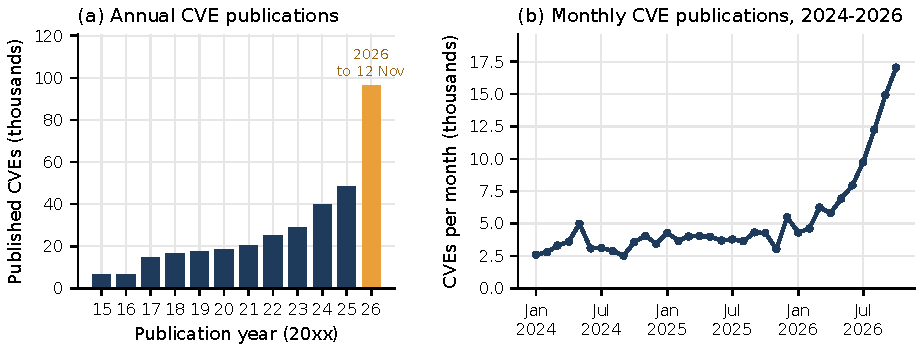
\includegraphics[width=\textwidth]{fig02_cve_volume.pdf}
\caption{CVE publication volume. (a) Annual totals; the 2026 bar covers 1 January to 12 November. (b) Monthly totals, January 2024 to October 2026. Source: CVE List V5 snapshot, author calculations.}
\label{fig:volume}
\end{figure}

The surge is not confined to open-source projects. Table~\ref{tab:vendor} and Figure~\ref{fig:vendor} show that vulnerabilities assigned by large commercial vendors' own CNAs rose by factors of 33 (Google Chrome), 13 (Oracle), 4 (Microsoft) and 2 (Apple). For banks, this matters more than the total: these vendors supply the browsers, operating systems, office software, databases and middleware on which every bank runs. The patch workload of a bank's IT function scales with these counts. A doubling or quadrupling of vendor advisories in a single year is an operational shock even before any vulnerability is exploited.

\begin{figure}[!htbp]
\centering
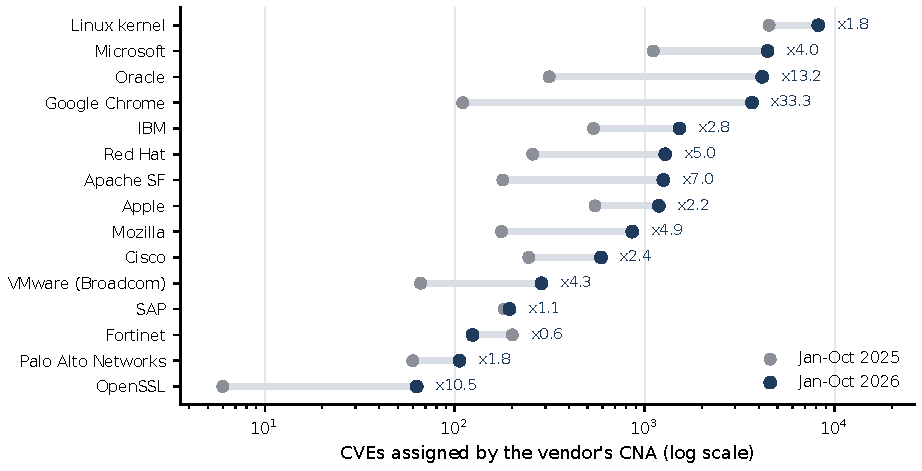
\includegraphics[width=\textwidth]{fig03_vendor_surge.pdf}
\caption{CVEs assigned by selected CNAs, January--October 2025 vs.\ January--October 2026 (log scale). Labels show the ratio.}
\label{fig:vendor}
\end{figure}

\begin{table}[!htbp]
\centering
\caption{CVE counts by assigning CNA, January--October, with credit coverage and AI-credited CVEs in 2026.}
\label{tab:vendor}
\small
\begin{tabular}{lrrrrr}
\toprule
Assigning CNA & Jan--Oct 2025 & Jan--Oct 2026 & Ratio & Credited (\%) & AI-credited \\
\midrule
Linux kernel & 4,516 & 8,197 & 1.8 & 0 & 0 \\
Microsoft & 1,108 & 4,437 & 4.0 & 0 & 0 \\
Oracle & 314 & 4,154 & 13.2 & 0 & 0 \\
Google Chrome & 110 & 3,667 & 33.3 & 0 & 0 \\
IBM & 538 & 1,524 & 2.8 & 15 & 1 \\
Red Hat & 257 & 1,282 & 5.0 & 73 & 176 \\
Apache SF & 179 & 1,252 & 7.0 & 90 & 177 \\
Apple & 547 & 1,187 & 2.2 & 0 & 0 \\
Mozilla & 176 & 859 & 4.9 & 100 & 95 \\
Cisco & 245 & 589 & 2.4 & 17 & 0 \\
VMware (Broadcom) & 66 & 286 & 4.3 & 5 & 0 \\
SAP & 182 & 194 & 1.1 & 0 & 0 \\
Fortinet & 201 & 124 & 0.6 & 0 & 0 \\
Palo Alto Networks & 60 & 106 & 1.8 & 97 & 1 \\
OpenSSL & 6 & 63 & 10.5 & 100 & 30 \\
\bottomrule
\end{tabular}
\end{table}

\paragraph{What caused the shock?} The data cannot attribute the surge to AI on their own. The CNAs with the largest increases (Microsoft, Chrome, Oracle) publish no credits, so their records do not say who or what found the bugs. Three observations nevertheless point to AI-assisted discovery as a major contributor. First, the timing coincides with the deployment of agentic security researchers and restricted-access defensive programmes in late 2025 and 2026 \citep{openai2025aardvark,deepmind2025codemender,anthropic2026glasswing}. Second, among CNAs that do publish credits, AI-credited records rose from almost none to hundreds per month over the same period (Section~\ref{sec:ai}). Third, the CNAs that publish credits and grew fastest---Apache (+177 AI-credited CVEs in 2026), Red Hat (+176), Mozilla (+95) and OpenSSL (+30)---have substantial AI-credited shares. Other factors, including CNA process changes and the expansion of CNAs such as VulnCheck and GitHub, also contribute. We treat AI as a likely but unquantified driver of the commercial-vendor surge.

%=====================================================================
\section{Results II: AI in vulnerability discovery}\label{sec:ai}

\subsection{Scale and trajectory}
We identify 1,598 AI-credited CVEs: 665 in Tier~1 (an AI system named) and 933 in Tier~2 (an AI-native organisation credited). Seven appear before 2025, 151 in 2025 and 1,440 in 2026. The first Tier~1 credit in our data is dated 20 March 2025 (XBOW, an autonomous penetration-testing system, credited on an Apache CVE). Figure~\ref{fig:aimonthly} shows that monthly counts grew at about 18.6\% per month (s.e.\ 3.8 percentage points) between July 2025 and October 2026, a doubling time of about 4.1 months. In October 2026, AI-credited CVEs were 4.1\% of all CVEs that carry any credit and 2.0\% of all CVEs. Because the largest commercial CNAs publish no credits, the true share is higher.

\begin{figure}[!htbp]
\centering
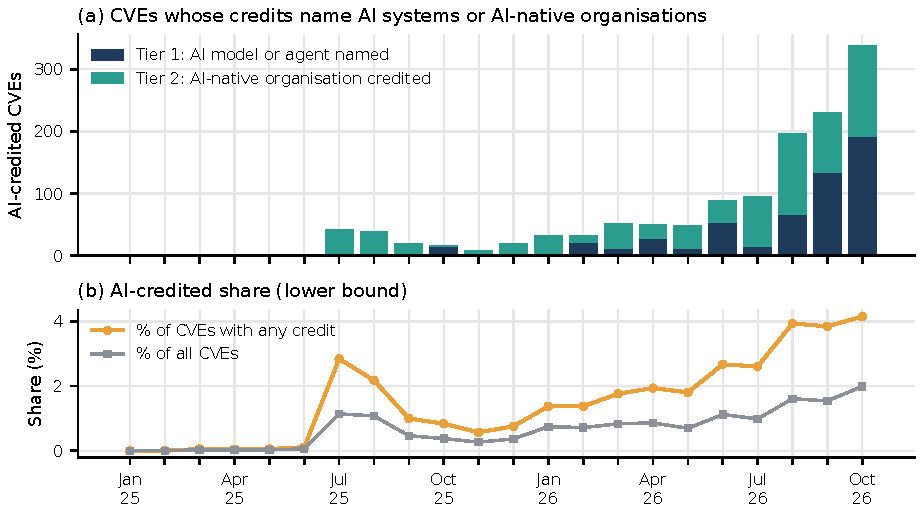
\includegraphics[width=\textwidth]{fig04_ai_monthly.pdf}
\caption{AI-credited CVEs per month, January 2025 to October 2026. (a) Counts by tier. (b) Share of CVEs with any credit, and share of all CVEs. Both shares are lower bounds.}
\label{fig:aimonthly}
\end{figure}

\subsection{Who is credited and what they find}
Table~\ref{tab:developers} and Figure~\ref{fig:aibreak}(a) show a concentrated field. Credits naming Anthropic's Claude models and agents (510) and the AI-native firm AISLE (438) dominate, followed by OpenAI (196, of which 74 name Codex Security or a GPT model), ZAST.AI (171) and a long tail of smaller AI security firms. Google's Big Sleep appears on 18 CVEs. These include CVE-2025-6965 in SQLite, which the vendor described as otherwise known only to threat actors---an example of AI \emph{pre-empting} exploitation (Table~\ref{tab:milestones}).

\begin{table}[!htbp]
\centering
\begin{minipage}[t]{0.45\textwidth}
\centering
\caption{AI-credited CVEs by credited developer. A CVE can credit more than one developer.}
\label{tab:developers}
\small
\resizebox{\textwidth}{!}{\begin{tabular}{lrrr}
\toprule
Developer credited & Tier 1 & Tier 2 & Total \\
\midrule
Anthropic & 510 & 0 & 510 \\
AISLE & 0 & 438 & 438 \\
OpenAI & 74 & 122 & 196 \\
ZAST.AI & 0 & 171 & 171 \\
Other AI tools/orgs & 74 & 28 & 102 \\
WatchGuard & 0 & 28 & 28 \\
Striga & 0 & 28 & 28 \\
depthfirst & 0 & 22 & 22 \\
Horizon3.ai & 0 & 21 & 21 \\
Mopmonk AI & 0 & 20 & 20 \\
Google & 18 & 0 & 18 \\
CodeAnt AI & 0 & 18 & 18 \\
Other (7 developers) & 8 & 49 & 57 \\
\bottomrule
\end{tabular}}
\end{minipage}\hfill
\begin{minipage}[t]{0.52\textwidth}
\centering
\caption{Severity of 2026 CVEs by credit type (maximum CVSS base score where available).}
\label{tab:severity}
\small
\resizebox{\textwidth}{!}{\begin{tabular}{lrrrr}
\toprule
Group (CVEs published in 2026) & Scored & Mean CVSS & High+ (\%) & Critical (\%) \\
\midrule
AI-credited (tier 1) & 593 & 7.07 & 56.8 & 9.8 \\
AI-credited (tier 2) & 796 & 6.83 & 47.6 & 9.0 \\
Human-credited & 40,338 & 6.98 & 51.3 & 12.4 \\
All other 2026 CVEs & 89,689 & 7.07 & 56.8 & 12.4 \\
\bottomrule
\end{tabular}}
\vspace{4pt}
\parbox{\textwidth}{\footnotesize Mann--Whitney test, all AI-credited vs.\ human-credited: $p=0.66$.}
\end{minipage}
\end{table}

\begin{figure}[!htbp]
\centering
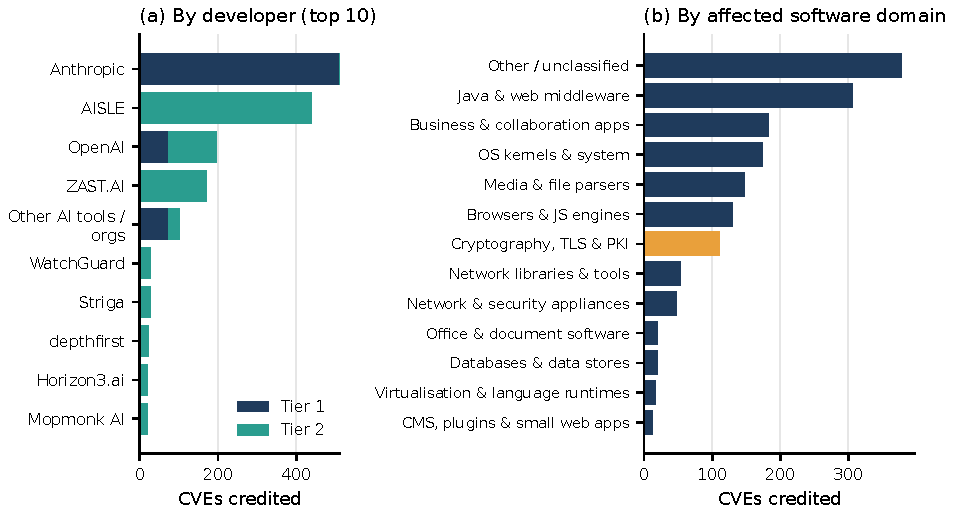
\includegraphics[width=\textwidth]{fig05_ai_breakdown.pdf}
\caption{AI-credited CVEs (a) by credited developer (top 10) and (b) by affected software domain. Cryptography, TLS and PKI libraries are highlighted.}
\label{fig:aibreak}
\end{figure}

The affected software is mostly open-source infrastructure: Java and web middleware (largely Apache projects), operating-system components, media parsers, browsers, and business and collaboration applications (Figure~\ref{fig:aibreak}b). One domain stands out for banking: 111 AI-credited CVEs affect cryptographic, TLS and PKI libraries. These comprise 52 in Bouncy Castle, the dominant Java cryptography provider in enterprise and banking software; 33 in OpenSSL; and 25 in wolfSSL/wolfSSH, which is widely embedded in devices. Cryptographic libraries are the software layer of the trust anchors discussed in Section~\ref{sec:hardware}.

\paragraph{Severity.} AI-credited vulnerabilities are not trivial. In 2026, Tier~1 CVEs had a mean maximum CVSS score of 7.07, with 56.8\% rated high or critical, against 6.98 and 51.3\% for human-credited CVEs (Table~\ref{tab:severity}). The difference between all AI-credited and human-credited CVEs is not significant ($p=0.66$). AI systems find vulnerabilities of the same severity as human researchers.

\subsection{From AI discovery to exploitation}
Fifteen AI-credited CVEs have entered the KEV catalogue (Table~\ref{tab:aikev}). Three features stand out. First, the median lag from publication to KEV listing is 17 days; these were exploited as n-days after disclosure rather than as zero-days. Second, seven of the fifteen were found by Horizon3.ai, an offensive-security firm that focuses on enterprise products attackers prize, so the apparent exploitation rate of AI-credited CVEs (9.4 per 1,000, against 1.5 for human-credited CVEs over 2023--2026) reflects \emph{what} these firms look at more than \emph{how} they find it. Third, only one Tier~1 CVE (Brotli, credited to OpenAI Codex Security) has been exploited, and none of the 86 Tier~1 CVEs in the censoring-robust cohort was listed within 180 days. Products in this set---SolarWinds Web Help Desk, SimpleHelp, JFrog Artifactory, Apache ActiveMQ and Tomcat, Palo Alto Expedition, Langflow and PHP---are typical of enterprise estates, including banks.

\begin{table}[!htbp]
\centering
\caption{AI-credited CVEs that entered the KEV catalogue.}
\label{tab:aikev}
\scriptsize
\resizebox{\textwidth}{!}{\begin{tabular}{llllrr}
\toprule
CVE & Product & Credited AI party & Published & KEV listed & Lag (d) \\
\midrule
CVE-2023-27524 & Apache Superset & Horizon3.ai & 2023-04-24 & 2024-01-08 & 259 \\
CVE-2024-9465 & Palo Alto Networks Expedition & Horizon3.ai & 2024-10-09 & 2024-11-14 & 36 \\
CVE-2025-3248 & Langflow Langflow & Horizon3.ai & 2025-04-07 & 2025-05-05 & 28 \\
CVE-2025-5086 & Dassault Systèmes DELMIA Apriso & Hacktron & 2025-06-02 & 2025-09-11 & 101 \\
CVE-2025-40551 & SolarWinds Web Help Desk & Horizon3.ai & 2026-01-28 & 2026-02-03 & 6 \\
CVE-2025-40536 & SolarWinds Web Help Desk & Horizon3.ai & 2026-01-28 & 2026-02-12 & 15 \\
CVE-2026-34197 & Apache ActiveMQ & Horizon3.ai & 2026-04-07 & 2026-04-16 & 9 \\
CVE-2026-48558 & SimpleHelp  SimpleHelp & Horizon3.ai & 2026-06-12 & 2026-06-29 & 17 \\
CVE-2026-34486 & Apache Tomcat & Striga & 2026-04-09 & 2026-08-04 & 117 \\
CVE-2026-66384 & JFrog Artifactory & OpenAI (organisation) & 2026-08-12 & 2026-08-27 & 15 \\
CVE-2026-42016 & JFrog Artifactory & OpenAI (organisation) & 2026-07-27 & 2026-09-11 & 46 \\
CVE-2026-5430 & WSO2 Multiple Products & Hacktron & 2026-08-06 & 2026-09-24 & 49 \\
CVE-2026-109618 & PHP Group PHP & OpenAI (organisation) & 2026-10-21 & 2026-10-26 & 5 \\
CVE-2026-109619 & PHP Group PHP & OpenAI (organisation) & 2026-10-21 & 2026-10-26 & 5 \\
CVE-2026-111497 & Google Brotli & Codex Security / Aardvark & 2026-10-22 & 2026-10-27 & 5 \\
\bottomrule
\end{tabular}}
\end{table}

\paragraph{Answer to RQ1.} AI-credited discovery went from negligible to roughly 2--4\% of credited CVEs in eighteen months and is doubling every four months. The publicly visible activity is overwhelmingly defensive or coordinated: AI developers, AI-native security firms and open-source maintainers disclosing and fixing bugs. Offensive use is documented in threat reports \citep{microsoft2024threat,anthropic2025espionage}, but does not appear in vulnerability records, because attackers do not credit themselves. The number of people ``using AI to hunt for zero-days'' therefore cannot be counted directly. The observable footprint is large and growing, and the capability it reveals is available, with some lag, to attackers.

%=====================================================================
\section{Results III: exploitation of commercial software}\label{sec:exploitation}

\subsection{What gets exploited}
Of the 1,779 KEV entries, 263 vendors appear among additions since 2022; the ten most frequent (led by Microsoft, Cisco, Adobe, Apple, Google and Oracle) account for 51.8\%. Figure~\ref{fig:kevcat} shows how the composition of additions has shifted. Enterprise perimeter and network infrastructure---VPN, firewall, application-delivery and router platforms from vendors such as Fortinet, Palo Alto Networks, Citrix, Ivanti, Cisco and SonicWall---rose from 14.6\% of additions in 2022 to 21.0\% in 2026. IT-management and remote-access tools rose to 14.6\% in 2026, from 1.8\% in 2022. Browsers and plug-ins declined. A new category appeared: AI and automation platforms (for example Langflow and LiteLLM), with 12 entries, 11 of them added in 2026. The Herfindahl index of exploitation across vendors fell from 0.114 in 2022 to 0.035 in 2026: attackers now exploit a wider range of vendors.

\begin{figure}[!htbp]
\centering
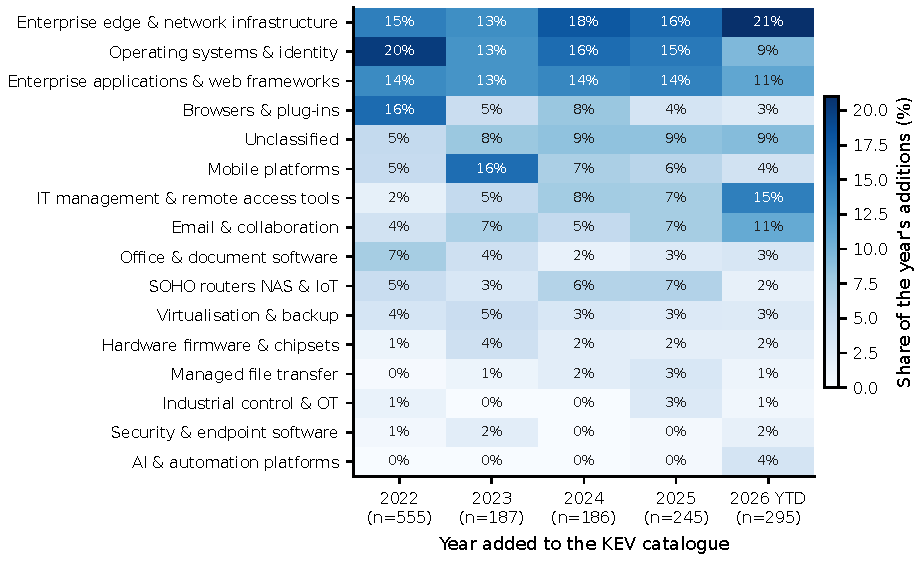
\includegraphics[width=\textwidth]{fig06_kev_categories.pdf}
\caption{Composition of KEV additions by product category and year (share of the year's additions). 2021 is omitted because the catalogue launched with a back-filled list.}
\label{fig:kevcat}
\end{figure}

\subsection{How fast exploitation follows disclosure}
Table~\ref{tab:lags} and Figure~\ref{fig:lags}(a) report listing lags. In the censoring-robust cohort, the median lag has been between 4 and 6 days for every publication year since 2022. Between 51.5\% and 64.9\% of listed vulnerabilities were listed within a week, and 28--39\% were listed on or before the day the CVE was published. We find no further compression after 2022 (Kendall's $\tau=0.035$, $p=0.20$). Industry studies report that the average time-to-exploit fell from about a month to a few days during 2021--2023 \citep{mandiant2024tte}; our data suggest that the compression has since plateaued at that low level. This does not support the stronger form of our hypothesis H2 (continuing compression). The weaker form holds: the window is already too short for monthly patch cycles.

\begin{table}[!htbp]
\centering
\caption{KEV listing lags by CVE publication year (censoring-robust cohort), and zero-day proxy counts vs.\ published industry counts.}
\label{tab:lags}
\small
\begin{tabular}{lrrrrrrr}
\toprule
 & \multicolumn{5}{c}{Cohort: listed within 180 days} & \multicolumn{2}{c}{Zero-day counts} \\
\cmidrule(lr){2-6}\cmidrule(lr){7-8}
CVE year & $n$ & Median lag & IQR & $\le 0$ d (\%) & $\le 7$ d (\%) & Proxy & Reported \\
\midrule
2021$^a$ & 16 & 20.0 & [0, 143] & 31.2 & 50.0 & 8 & -- \\
2022 & 99 & 6.0 & [-1, 45] & 39.4 & 51.5 & 51 & 55 \\
2023 & 134 & 4.0 & [0, 14] & 34.3 & 64.9 & 87 & 97 \\
2024 & 132 & 4.5 & [0, 36] & 29.5 & 59.1 & 78 & 75 \\
2025 & 175 & 5.0 & [0, 33] & 28.0 & 55.4 & 97 & -- \\
2026$^b$ & 65 & 5.0 & [0, 15] & 27.7 & 56.9 & 128 & -- \\
\bottomrule
\end{tabular}
\vspace{2pt}
\parbox{0.95\textwidth}{\footnotesize $^a$~November--December 2021 only. $^b$~CVEs published to mid-May 2026. ``Proxy'' counts all early-listed post-launch entries by publication year. ``Reported'': industry counts of in-the-wild zero-days as reported by Mandiant (2022) and Google (2023, 2024) \citep{mandiant2023zeroday,google2024zeroday,gtig2025zeroday}. Google Project Zero's own count for 2022 was 41. Benchmark figures should be verified against the original reports.}
\end{table}

\begin{figure}[!htbp]
\centering
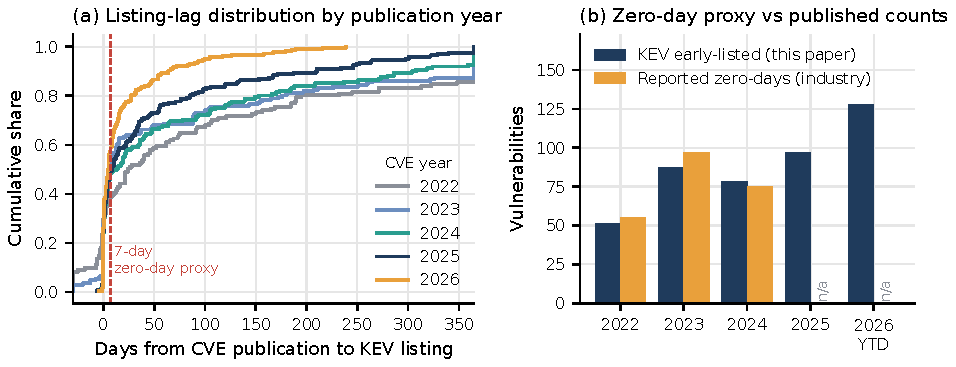
\includegraphics[width=\textwidth]{fig07_lags.pdf}
\caption{(a) Cumulative distribution of days from CVE publication to KEV listing, by publication year (clipped to $[-30,365]$). (b) Annual count of early-listed vulnerabilities (zero-day proxy) vs.\ industry-reported zero-day counts.}
\label{fig:lags}
\end{figure}

\paragraph{Validating the zero-day proxy.} Early-listed counts by publication year were 51, 87 and 78 for 2022--2024, against reported in-the-wild zero-day counts of 55, 97 and 75---a mean absolute deviation of 7.2\% (Figure~\ref{fig:lags}b). The two series measure overlapping but not identical sets, so the agreement supports using the proxy for levels and trends, not for individual classification. On this proxy, zero-day-like exploitation rose to 97 in 2025 and 128 in 2026 to date, the highest in the series.

\subsection{Exploitation has grown more slowly than discovery}
KEV additions rose from 186 in 2024 to 245 in 2025 and 295 in 2026 to 10 November. Disclosure grew much faster, so the share of new CVEs that are exploited fell (Table~\ref{tab:k180}). In the censoring-robust cohort, an average of 3.89 of every 1,000 CVEs published between 2022 and 2025 were listed within 180 days, against 2.62 per 1,000 in the first half of 2026. If the disclosure shock is substantially AI-driven, the defenders' side of AI is currently ahead: vulnerabilities are being found and fixed faster than attackers are converting them into exploitation. This is our hypothesis H1. The same numbers carry a warning. A falling exploitation \emph{rate} on a quadrupling \emph{base} still means more exploited vulnerabilities in absolute terms, and the defenders' patch workload has multiplied.

\begin{table}[!htbp]
\centering
\caption{KEV listings within 180 days per 1,000 CVEs, by publication half-year.}
\label{tab:k180}
\small
\begin{tabular}{lrrr}
\toprule
Publication half-year & CVEs & In KEV within 180 d & Per 1,000 \\
\midrule
2022H1 & 12,343 & 53 & 4.29 \\
2022H2 & 12,656 & 46 & 3.63 \\
2023H1 & 14,120 & 55 & 3.90 \\
2023H2 & 14,727 & 79 & 5.36 \\
2024H1 & 20,349 & 54 & 2.65 \\
2024H2 & 19,575 & 78 & 3.98 \\
2025H1 & 23,642 & 96 & 4.06 \\
2025H2 & 24,508 & 79 & 3.22 \\
2026H1 & 24,815 & 65 & 2.62 \\
\bottomrule
\end{tabular}
\end{table}

\paragraph{Answer to RQ2.} The commercial products exploited most often, and most often as zero-days, are perimeter devices (59.9\% zero-day-like), operating systems (61.8\%), browsers (93.2\%), mobile platforms (70.8\%) and managed file transfer (64.7\%). Products with the heaviest ransomware association are mail and collaboration servers (37.2\%), MFT (35.3\%) and IT-management tools (29.3\%) (Table~\ref{tab:profile}). Well-known named campaigns in these categories---MOVEit, GoAnywhere, Accellion FTA, Exchange ProxyLogon, Citrix NetScaler, Ivanti Connect Secure, Fortinet FortiOS, SharePoint and Oracle E-Business Suite---are the specific products behind these aggregates.

%=====================================================================
\section{Hardware trust anchors and hardware wallets}\label{sec:hardware}

RQ3 asks whether zero-days in hardware wallets matter for banks. Table~\ref{tab:hardware} summarises 11 cases. Hardware wallets share their building blocks with banking infrastructure: secure elements, microcontrollers, firmware and cryptographic libraries. These same blocks protect payment cards, PIN and payment HSMs, FIDO keys used by bank staff, TPMs in servers, and the secure enclaves of the phones that run mobile banking.

\begin{table}[!htbp]
\centering
\caption{Hardware trust-anchor cases and their banking analogues (author-coded from public research and reporting).}
\label{tab:hardware}
\scriptsize
\begin{tabular}{p{0.05\textwidth}p{0.19\textwidth}p{0.24\textwidth}p{0.16\textwidth}p{0.24\textwidth}}
\toprule
Year & Target & Attack class & Access required & Banking analogue \\
\midrule
2010 & EMV chip-and-PIN cards & Protocol logic flaw (PIN verification bypass) & Physical card and modified terminal & Card-present payments \\
2017 & Infineon RSA key generation (ROCA) & Weak key generation (factorable public keys) & Remote (public key only) & Smart cards; tokens; TPMs; national ID used for e-banking \\
2018 & Trezor; Ledger; KeepKey (wallet.fail) & Fault injection and supply-chain tampering & Physical device & Hardware authentication tokens; HSM tamper resistance \\
2019 & Apple BootROM A5-A11 (checkm8) & Unpatchable BootROM memory-safety bug & Physical (USB) & Integrity of phones running mobile banking \\
2019 & General-purpose HSM (research disclosure) & Firmware memory-safety bugs enabling key extraction & Network/API access to HSM & Payment and PIN HSMs in bank data centres \\
2019 & Intel fTPM and STMicro TPM (TPM-Fail) & Timing side channel on ECDSA & Local or network timing & Server attestation and key storage \\
2020 & Trezor One/T seed extraction & Voltage glitching of microcontroller & Physical (minutes) & Stolen token or HSM scenarios \\
2021 & EMV contactless (Visa PIN bypass) & Protocol flaw allowing PIN bypass & Physical proximity (relay) & Contactless payments \\
2023 & Ledger Connect Kit & Malicious library version published via compromised account & Remote & Banking SDKs and front-end libraries \\
2024 & Infineon ECDSA in YubiKey 5 (EUCLEAK) & Electromagnetic side channel & Physical (lab equipment) & FIDO keys used by bank staff \\
2025 & Bybit cold-wallet signing (Safe interface) & Manipulated transaction display (blind signing) & Remote (supplier compromise) & Maker-checker payment approval screens \\
\bottomrule
\end{tabular}
\end{table}

Three lessons follow. First, six of the eleven cases require physical access to the device: glitching, side channels, or a USB connection to a boot ROM. Such attacks do not scale to a remote campaign against a bank, but they matter for stolen tokens, insider threats and supply-chain tampering. Second, the remote cases are the dangerous ones, and they sit in software around the hardware. ROCA was a flaw in key generation in a secure-element library, exploitable from a public key alone \citep{nemec2017roca}. The Ledger Connect Kit incident was a compromised software dependency. The 2025 Bybit theft manipulated the transaction-display layer of a multisig signing workflow, so that signers approved a transfer they did not intend. The banking analogue of this last case is the maker--checker approval screen for high-value payments. Third, AI discovery is now active in exactly this software layer: 111 AI-credited CVEs affect cryptographic libraries (Section~\ref{sec:ai}).

\paragraph{Answer to RQ3.} Hardware-wallet zero-days are relevant to banks less through the wallets themselves than through common components and patterns. These are secure-element libraries (ROCA-type flaws), HSM firmware \citep{campana2019hsm}, payment-card protocols \citep{murdoch2010chip,basin2021emv} and transaction-display integrity in signing workflows. Banks and central banks that hold or plan to hold digital assets, issue tokenised deposits or pilot CBDC with offline hardware wallets inherit these risks directly.

%=====================================================================
\section{Financial-sector exposure}\label{sec:exposure}

\subsection{Bank-weighted exploitation pressure}
Weighting KEV categories by their relevance to bank estates (Figure~\ref{fig:pressure}, Table~\ref{tab:profile}) puts enterprise perimeter infrastructure first ($\Pi=162$, of which 97 zero-day-like), followed by operating systems and identity (91.7), enterprise applications and web frameworks (81.6), IT-management and remote-access tools (73.8), and mail and collaboration (70.2). The ranking is robust to the weights: across 2,000 random perturbations of $\pm0.3$, the median Kendall rank correlation with the baseline is 0.88 (5th percentile 0.80), and it is 0.83 under uniform weights.

\begin{figure}[!htbp]
\centering
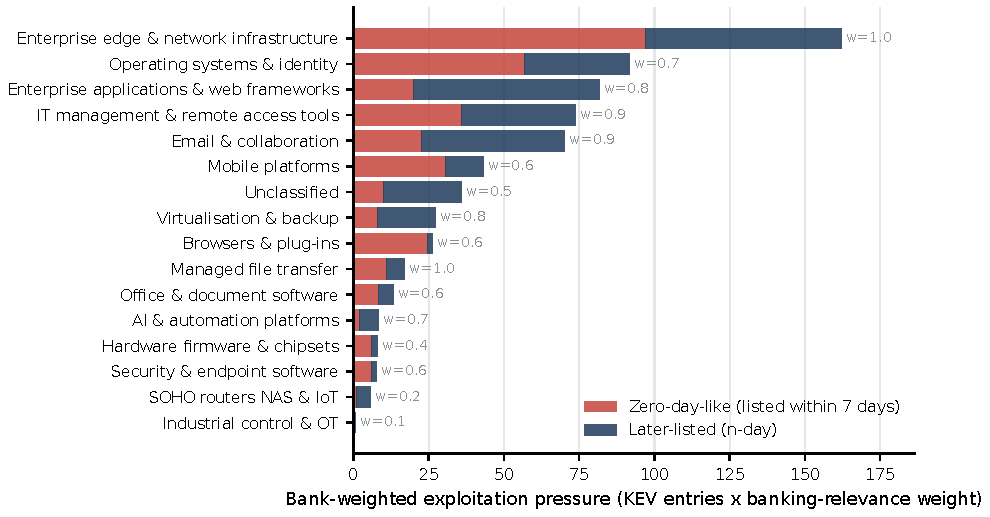
\includegraphics[width=\textwidth]{fig08_bank_pressure.pdf}
\caption{Bank-weighted exploitation pressure by product category, KEV entries for CVEs published since November 2021. Red: zero-day-like (listed within seven days); blue: later-listed. $w$: banking-relevance weight.}
\label{fig:pressure}
\end{figure}

\begin{table}[!htbp]
\centering
\caption{Exploitation profile of product categories (KEV entries for CVEs published since November 2021).}
\label{tab:profile}
\scriptsize
\resizebox{\textwidth}{!}{\begin{tabular}{lrrrrrr}
\toprule
Product category & $n$ & Zero-day-like (\%) & Median lag (d) & Ransomware (\%) & Weight $w_c$ & Pressure \\
\midrule
Enterprise edge \& network infrastructure & 162 & 59.9 & 5.0 & 21.0 & 1.0 & 162.0 \\
Operating systems \& identity & 131 & 61.8 & 0.0 & 20.6 & 0.7 & 91.7 \\
Enterprise applications \& web frameworks & 102 & 24.5 & 38.5 & 21.6 & 0.8 & 81.6 \\
IT management \& remote access tools & 82 & 48.8 & 9.0 & 29.3 & 0.9 & 73.8 \\
Email \& collaboration & 78 & 32.1 & 23.0 & 37.2 & 0.9 & 70.2 \\
Mobile platforms & 72 & 70.8 & 1.0 & 0.0 & 0.6 & 43.2 \\
Unclassified & 72 & 27.8 & 23.0 & 12.5 & 0.5 & 36.0 \\
Virtualisation \& backup & 34 & 29.4 & 24.5 & 23.5 & 0.8 & 27.2 \\
Browsers \& plug-ins & 44 & 93.2 & 1.0 & 2.3 & 0.6 & 26.4 \\
Managed file transfer & 17 & 64.7 & 4.0 & 35.3 & 1.0 & 17.0 \\
Office \& document software & 22 & 63.6 & 3.0 & 9.1 & 0.6 & 13.2 \\
AI \& automation platforms & 12 & 25.0 & 29.5 & 8.3 & 0.7 & 8.4 \\
Hardware firmware \& chipsets & 20 & 75.0 & 2.0 & 5.0 & 0.4 & 8.0 \\
Security \& endpoint software & 13 & 76.9 & 2.0 & 15.4 & 0.6 & 7.8 \\
SOHO routers NAS \& IoT & 29 & 17.2 & 48.0 & 3.4 & 0.2 & 5.8 \\
Industrial control \& OT & 8 & 12.5 & 85.0 & 0.0 & 0.1 & 0.8 \\
\bottomrule
\end{tabular}}
\end{table}

\subsection{What the incident record shows}
Table~\ref{tab:incsummary} and Figure~\ref{fig:incidents} summarise the 33 curated incidents (full list in Table~\ref{tab:incidents}). About half (17) began with stolen credentials, fraud, social engineering or misconfiguration, as in Bangladesh Bank 2016, JPMorgan Chase 2014 and Capital One 2019. Five involved a zero-day. In every one of the five, the zero-day was in a widely used commercial product rather than in banking software. Three were in MFT appliances (Accellion FTA, which reached the Reserve Bank of New Zealand; GoAnywhere; MOVEit), one was in on-premise Exchange (the European Banking Authority) and one was in a document reader, used against a security vendor serving banks (RSA, 2011). Three cases were supply-chain compromises (NotPetya, SolarWinds Orion, Bybit), and three exploited known n-days in perimeter devices or browsers (for example Travelex through an unpatched Pulse Secure VPN). One, the 2024 CrowdStrike update failure, was a non-malicious common-mode failure; it shows how a single shared component can disrupt banks and payment services worldwide within hours.

\begin{table}[!htbp]
\centering
\caption{Initial-vector classes in the curated incident set (descriptive; purposive sample).}
\label{tab:incsummary}
\small
\begin{tabular}{lrrrr}
\toprule
Initial-vector class & Cases & Share (\%) & Central bank / supervisor & Thailand \\
\midrule
Credentials, fraud or misconfiguration & 17 & 51.5 & 2 & 4 \\
Zero-day in commercial product & 5 & 15.2 & 2 & 0 \\
Vector not disclosed & 4 & 12.1 & 2 & 0 \\
Known (n-day) vulnerability & 3 & 9.1 & 0 & 0 \\
Supply-chain compromise & 3 & 9.1 & 1 & 0 \\
Non-malicious common-mode failure & 1 & 3.0 & 0 & 0 \\
\midrule
Total & 33 & 100.0 & 7 & 4 \\
\bottomrule
\end{tabular}
\end{table}

\begin{figure}[!htbp]
\centering
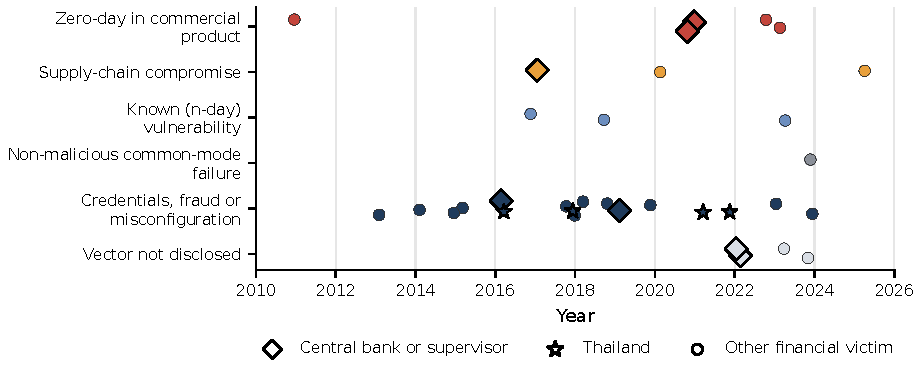
\includegraphics[width=\textwidth]{fig09_incidents.pdf}
\caption{Curated financial-sector incidents by year and initial-vector class. Diamonds: central banks or supervisors; stars: Thailand.}
\label{fig:incidents}
\end{figure}

Seven of the 33 cases hit central banks or supervisors. Their pattern is instructive: the RBNZ and EBA intrusions came through file-transfer and mail systems---commodity corporate IT---not through settlement systems. Bangladesh Bank was compromised in the environment around its payment-messaging interface. Bank Indonesia and the Bank of Zambia suffered ransomware.

\subsection{Would AI-discovered zero-days be used against banks?}
The evidence supports four statements. (i) Financial institutions are attractive targets for both financially motivated and state-linked actors. Some state-linked groups have a long record of attacks on banks and crypto firms (Bangladesh Bank, Bybit), and the AI-orchestrated campaign reported in 2025 reportedly included financial institutions among its intended targets \citep{anthropic2025espionage}. (ii) Zero-days reach banks through the commercial products that banks share with every other sector. An attacker does not need a ``banking zero-day''; an MFT or VPN zero-day reaches hundreds of banks at once. (iii) As AI lowers the cost of discovery, the scarcity that limited zero-day use to a few actors weakens. Mass-exploitation crews of the MOVEit type are the actors most likely to benefit, because their business model already converts one zero-day into many victims. (iv) We found no publicly documented case, up to our snapshot, of an AI-discovered zero-day used against a bank. Given the lags in public reporting and attackers' incentives not to disclose methods, this absence is weak evidence of safety.

\paragraph{Answer to RQ4.} The global banking system is exposed mainly through perimeter devices, MFT, IT-management tools, mail and collaboration servers, and shared service providers. AI-discovered zero-days are likely to be used against banks through these products. The likeliest form is mass exploitation and data extortion. Destructive attacks on payment systems are possible but less likely, because they require deeper access and invite a strong state response.

%=====================================================================
\section{Thailand}\label{sec:thailand}

\subsection{Institutional setting}
Thailand's financial system combines a concentrated commercial banking sector, in which a small number of domestic systemically important banks (D-SIBs) account for most deposits and payments, with state-owned specialised financial institutions (SFIs) that serve retail, rural, housing and SME segments. A large non-bank payment and e-money sector operates under the Payment Systems Act B.E.~2560 (2017) \citep{thailand2017payment}. Virtual banks were licensed in 2025 under a framework issued in 2024 \citep{bot2024virtual}, and digital-asset exchanges and custodians are supervised by the securities regulator. The core payment infrastructure comprises the BOT-operated RTGS system (BAHTNET), the retail real-time payment system (PromptPay and related services operated by National ITMX) and card switching. The Cybersecurity Act B.E.~2562 (2019) designates the banking and financial sector as critical information infrastructure \citep{thailand2019cyber}, and the Thai Bankers' Association operates a sector CERT (TB-CERT).

The four Thai cases in our incident set---ATM malware at a state-owned bank (2016), web-application data leaks at two large banks (2018), a card-not-present fraud wave (2021) and remote-access malware on customers' phones (2022--2023)---involved no zero-day. Thai institutions nevertheless run the same commercial perimeter, MFT, mail, IT-management and virtualisation products that appear in the KEV catalogue, so they sit in the path of the same global mass-exploitation waves.

\subsection{Targets and vulnerable groups}
Table~\ref{tab:thai} and Figure~\ref{fig:thai} report the group framework. Groups with the highest \emph{target} index are the D-SIBs, payment FMIs, shared IT and cloud providers, the BOT's corporate and supervisory IT, and SFIs. Groups with the highest \emph{vulnerability} index are retail customers and their devices, payment and e-money providers, virtual banks, shared providers, digital-asset firms and non-bank lenders. Combining the two, three groups rank highest: shared IT and cloud providers ($R=0.72$; in the top three in 86\% of robustness draws), D-SIBs (0.67; 73\%) and SFIs (0.59; 52\%). Digital-asset exchanges and custodians (0.56) and non-bank payment providers (0.52) follow.

\begin{table}[!htbp]
\centering
\caption{Thai group framework: scores ($A$ attractiveness, $S$ systemic importance, $E$ exposure, $K$ concentration, $D$ defensive capacity), risk $R$, rank, 90\% rank interval and probability of ranking in the top three across 10,000 robustness draws. Scores are structured author judgements about groups, not assessments of institutions.}
\label{tab:thai}
\scriptsize
\resizebox{\textwidth}{!}{\begin{tabular}{p{0.30\textwidth}rrrrrrrrr}
\toprule
Group & $A$ & $S$ & $E$ & $K$ & $D$ & $R$ & Rank & 90\% rank & P(top 3) \\
\midrule
Shared IT and cloud service providers to the sector & 4 & 5 & 4 & 5 & 3 & 0.72 & 1 & 1--5 & 86 \\
Large systemically important banks & 5 & 5 & 5 & 4 & 5 & 0.67 & 2 & 1--6 & 73 \\
Specialised financial institutions (state-owned) & 4 & 4 & 4 & 4 & 3 & 0.59 & 3 & 1--8 & 52 \\
Digital-asset exchanges and custodians & 5 & 2 & 5 & 4 & 3 & 0.56 & 4 & 1--10 & 32 \\
Non-bank payment and e-money providers & 3 & 3 & 5 & 4 & 2 & 0.52 & 5 & 2--10 & 25 \\
Retail customers and their mobile devices & 3 & 2 & 5 & 4 & 1 & 0.47 & 6 & 2--11 & 11 \\
Other domestic commercial banks & 3 & 3 & 4 & 4 & 3 & 0.44 & 7 & 3--11 & 8 \\
Virtual banks (licensed 2025) & 3 & 2 & 5 & 5 & 3 & 0.43 & 8 & 4--11 & 5 \\
Bank of Thailand corporate and supervisory IT & 4 & 4 & 3 & 3 & 4 & 0.43 & 9 & 3--11 & 5 \\
Payment FMIs (RTGS; retail switch; card switch) & 5 & 5 & 2 & 3 & 5 & 0.40 & 10 & 4--11 & 2 \\
Non-bank lenders and card companies & 2 & 2 & 4 & 4 & 2 & 0.32 & 11 & 6--12 & 0 \\
Foreign bank branches and subsidiaries & 3 & 2 & 3 & 3 & 4 & 0.27 & 12 & 9--12 & 0 \\
\bottomrule
\end{tabular}}
\end{table}

\begin{figure}[!htbp]
\centering
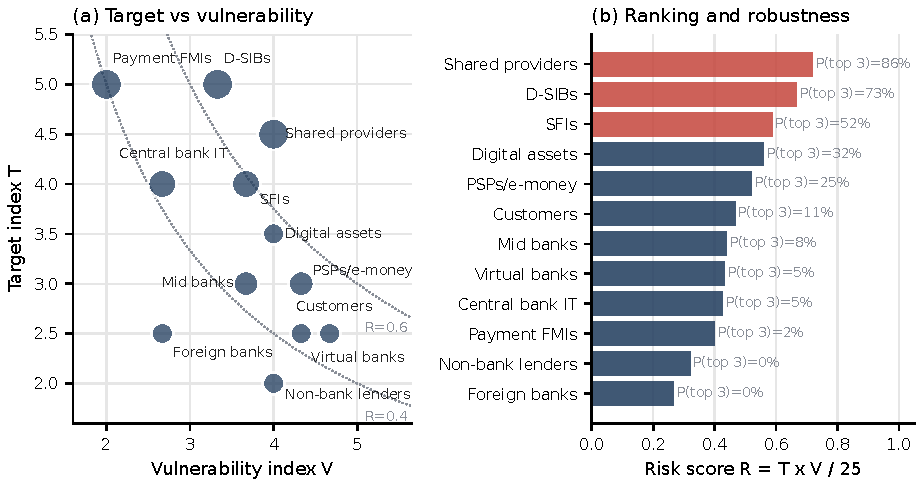
\includegraphics[width=\textwidth]{fig10_thai_groups.pdf}
\caption{Thai group framework. (a) Target index vs.\ vulnerability index; bubble size is systemic importance; dotted lines are iso-risk contours. (b) Risk score with the probability of ranking in the top three across robustness draws.}
\label{fig:thai}
\end{figure}

Three findings are robust to the perturbations. \emph{Shared providers rank at or near the top} because they combine one-to-many access with concentration: a single compromised outsourcer, cloud tenant or core-banking vendor creates correlated exposure across several banks, as the SolarWinds, MOVEit (via service providers) and CrowdStrike cases illustrate. \emph{D-SIBs are the main target but not the most vulnerable}: their defensive capacity offsets their exposure, yet their size makes any successful intrusion systemically relevant. \emph{Payment FMIs are high-value but low-vulnerability}: limited internet exposure and strong controls place them tenth, which is consistent with the absence of documented intrusions into core RTGS platforms in our incident set.

\paragraph{Answer to RQ5.} The likely \emph{targets} in Thailand are the D-SIBs, payment infrastructure, digital-asset platforms and the BOT itself. The groups most at \emph{risk} are shared IT providers, D-SIBs and SFIs. The most \emph{vulnerable} entry points are smaller non-bank payment firms, new virtual banks with concentrated cloud dependence, and customers' devices---the last mainly as a fraud channel that seldom needs zero-days. Whether Thai banks ``survive'' depends less on whether a Thailand-specific zero-day exists than on how quickly Thai institutions close exposure to global ones, and on whether a compromise at one shared provider can be contained.

%=====================================================================
\section{Scenario simulation}\label{sec:sim}

Tables~\ref{tab:simgroups}--\ref{tab:simparams} give the model's structure, calibration and scenarios. The base event rate of 86.7 exploited-vulnerability events per year across six enterprise layers comes from KEV. Edge and VPN products carry the highest rate (28.3 per year) and, with MFT, the highest zero-day share (0.61 and 0.67). For n-days, the median empirical KEV lag in these layers is 64 days. Scenario S0 represents conditions before 2022 (fewer zero-days, a 32-day time-to-exploit). S1 represents current conditions. S2 triples zero-day discovery and attacker throughput and shortens time-to-exploit to one day. S3 adds AI-enabled defence: patch times cut by 65\%, attack success reduced by 40\% through detection, and 30\% of bugs pre-empted. S4 adds vendor concentration to S2. S5 combines S3 with diversified vendor shares.

\begin{table}[!htbp]
\centering
\caption{Simulated institution groups (stylised; patch medians refer to critical internet-facing vulnerabilities).}
\label{tab:simgroups}
\small
\begin{tabular}{lrrrrrr}
\toprule
Group & Nodes & Payment share & Patch median (d) & Success $s_g$ & P(disrupt) & Attractiveness \\
\midrule
D-SIBs & 6 & 0.66 & 4 & 0.35 & 0.15 & 5 \\
Mid banks & 8 & 0.10 & 10 & 0.60 & 0.25 & 3 \\
Foreign banks & 12 & 0.06 & 7 & 0.45 & 0.20 & 3 \\
SFIs & 6 & 0.10 & 14 & 0.60 & 0.30 & 4 \\
Virtual banks & 3 & 0.01 & 5 & 0.60 & 0.30 & 3 \\
PSPs/e-money & 25 & 0.05 & 21 & 0.80 & 0.35 & 3 \\
Shared providers & 5 & 0.00 & 10 & 0.60 & 0.00 & 4 \\
Payment FMIs & 2 & 0.00 & 5 & 0.25 & 0.10 & 5 \\
\bottomrule
\end{tabular}
\end{table}

\begin{table}[!htbp]
\centering
\caption{Layer calibration from the KEV panel (CVEs published 2023--2025).}
\label{tab:simlayers}
\small
\resizebox{\textwidth}{!}{\begin{tabular}{lrrrrrr}
\toprule
Layer & Edge/VPN & MFT & Email/collab & IT mgmt/RMM & Virtualisation & Enterprise apps \\
\midrule
Event rate per year (KEV-calibrated) & 28.3 & 5 & 12.7 & 14.3 & 6.3 & 20 \\
Share exploited as zero-day & 0.61 & 0.67 & 0.26 & 0.37 & 0.26 & 0.18 \\
\bottomrule
\end{tabular}}
\end{table}

\begin{table}[!htbp]
\centering
\caption{Scenario parameters. $m_d$: discovery multiplier; $\tau$: zero-day copycat time-to-exploit (days); $\kappa$: n-day lag factor; $p_{\text{mass}}$: share of mass campaigns; $m_o$: attacker throughput; $\beta$: patch-time factor; $\delta$: success factor (detection); $\phi$: pre-emption share.}
\label{tab:simparams}
\small
\resizebox{\textwidth}{!}{\begin{tabular}{lrrrrrrrrl}
\toprule
Scenario & $m_d$ & $\tau$ & $\kappa$ & $p_{\text{mass}}$ & $m_o$ & $\beta$ & $\delta$ & $\phi$ & Vendor shares \\
\midrule
S0 Pre-2022 baseline & 0.6 & 32 & 1.3 & 0.25 & 1 & 1 & 1 & 0 & baseline \\
S1 Current (2023-26) & 1 & 5 & 1 & 0.35 & 1 & 1 & 1 & 0 & baseline \\
S2 AI offence & 3 & 1 & 0.2 & 0.5 & 3 & 1 & 1 & 0 & baseline \\
S3 AI offence + AI defence & 3 & 1 & 0.2 & 0.5 & 3 & 0.35 & 0.6 & 0.3 & baseline \\
S4 AI offence + concentration & 3 & 1 & 0.2 & 0.5 & 3 & 1 & 1 & 0 & concentrated \\
S5 AI offence + defence + diversified & 3 & 1 & 0.2 & 0.5 & 3 & 0.35 & 0.6 & 0.3 & diversified \\
\bottomrule
\end{tabular}}
\end{table}

\subsection{Results}
Table~\ref{tab:simresults} and Figure~\ref{fig:sim} report 4,000 simulated years per scenario. Under current conditions (S1), the model gives about 5.5 compromised institutions per year, a 26.6\% annual probability that at least one D-SIB is compromised, a 3.0\% probability of an FMI compromise and a 5.0\% probability of a systemic event. The absolute levels depend on assumptions. The comparisons across scenarios are the informative part:

\begin{itemize}
\item \textbf{AI offence multiplies systemic risk.} S2 raises the probability of a systemic event to 24.9\%, 5.0 times S1. Across the robustness grid (Table~\ref{tab:simrobust}), the ratio ranges from 4.0 to 6.8.
\item \textbf{AI defence recovers most of the loss.} S3 cuts the S2 probability to 9.8\%. Across the grid, defence removes 50--75\% of the systemic probability under AI offence (S3/S2 between 0.25 and 0.50).
\item \textbf{Concentration amplifies.} With a dominant vendor holding 60\% of each layer, S4 reaches 35.2\%, 36--64\% above S2 across the grid.
\item \textbf{Diversification helps less once defence is strong.} The S5/S3 ratio ranges from 0.67 to 1.15, so its benefit is not robust when defence is already effective.
\end{itemize}

\begin{table}[!htbp]
\centering
\caption{Simulation results (4,000 years per scenario). ``Systemic'': an event that disrupts $\ge10\%$ of payment value or any payment FMI.}
\label{tab:simresults}
\scriptsize
\resizebox{\textwidth}{!}{\begin{tabular}{lrrrrrr}
\toprule
Scenario & Events/yr & Compromised & P(D-SIB) \% & P(FMI) \% & P(systemic) \% [95\% CI] & RR vs S1 \\
\midrule
S0 Pre-2022 baseline & 52 & 2.9 & 15.9 & 1.4 & 2.9 [2.4, 3.4] & 0.59 \\
S1 Current (2023-26) & 87 & 5.5 & 26.6 & 3.0 & 5.0 [4.3, 5.6] & 1.00 \\
S2 AI offence & 260 & 28.5 & 82.2 & 17.2 & 24.9 [23.6, 26.2] & 5.03 \\
S3 AI offence + AI defence & 182 & 10.7 & 47.7 & 6.8 & 9.8 [8.9, 10.7] & 1.98 \\
S4 AI offence + concentration & 260 & 36.9 & 93.5 & 24.0 & 35.2 [33.7, 36.7] & 7.12 \\
S5 AI offence + defence + diversified & 182 & 9.1 & 41.3 & 5.3 & 8.8 [7.9, 9.7] & 1.78 \\
\bottomrule
\end{tabular}}
\end{table}

\begin{figure}[!htbp]
\centering
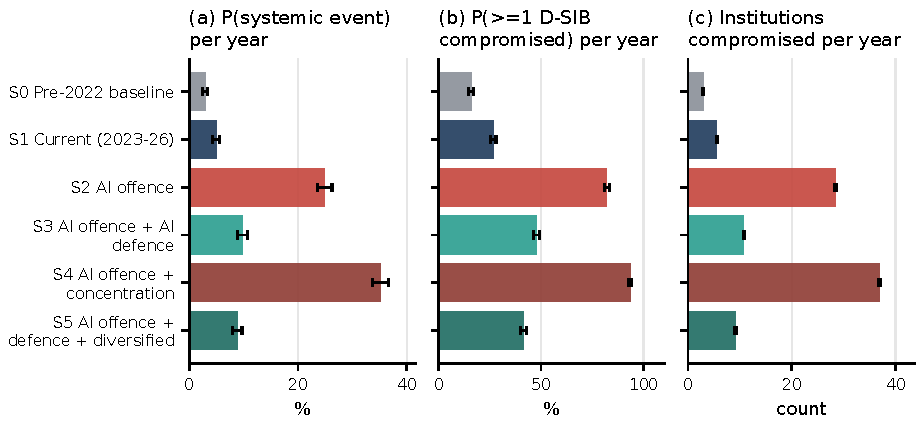
\includegraphics[width=\textwidth]{fig11_sim_scenarios.pdf}
\caption{Scenario outcomes with 95\% confidence intervals: (a) annual probability of a systemic event, (b) probability that at least one D-SIB is compromised, (c) institutions compromised per year.}
\label{fig:sim}
\end{figure}

Figure~\ref{fig:grid} varies the offence multiplier and the patch-time factor jointly. Offence dominates: at today's patch speed, the probability of a systemic event rises from 6\% to 45\% as the multiplier goes from 1 to 5. Faster patching alone has a modest effect. At a multiplier of 5, cutting patch times by 75\% lowers the probability only from 45\% to 40\%. When copycat exploitation starts within a day of disclosure and most damaging events begin as zero-days, the decisive defences act \emph{before} disclosure: pre-emptive discovery, smaller internet-facing exposure, detection and segmentation. This is the main operational lesson of the model.

\begin{figure}[!htbp]
\centering
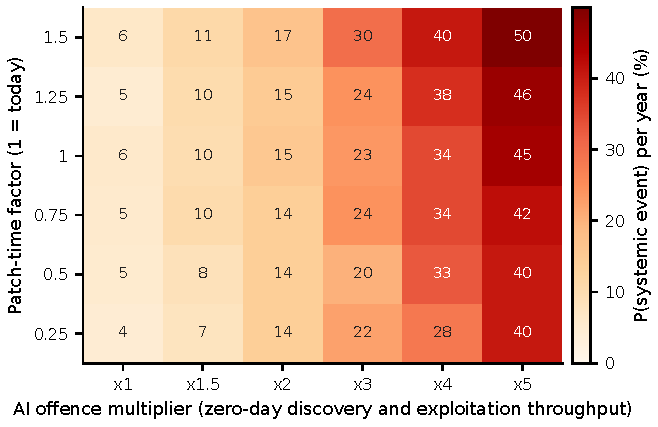
\includegraphics[width=0.78\textwidth]{fig12_sim_grid.pdf}
\caption{Annual probability of a systemic event (\%) by AI offence multiplier and patch-time factor (other parameters as in S2; 1,200 simulated years per cell).}
\label{fig:grid}
\end{figure}

\begin{table}[!htbp]
\centering
\caption{Robustness of scenario results to deployment probability $\rho$ and mass-campaign hit rate $c_{\text{mass}}$ (P(systemic) in \%, 1,000 years per cell).}
\label{tab:simrobust}
\scriptsize
\begin{tabular}{rrrrrrrrrrr}
\toprule
$\rho$ & $c_{\text{mass}}$ & S1 & S2 & S3 & S4 & S5 & S2/S1 & S3/S2 & S4/S2 & S5/S3 \\
\midrule
0.03 & 0.2 & 2.4 & 16.3 & 4.1 & 22.5 & 4.7 & 6.79 & 0.25 & 1.38 & 1.15 \\
0.03 & 0.3 & 4.0 & 16.0 & 6.6 & 26.3 & 4.4 & 4.00 & 0.41 & 1.64 & 0.67 \\
0.03 & 0.5 & 3.1 & 18.5 & 7.4 & 27.5 & 7.1 & 5.97 & 0.40 & 1.49 & 0.96 \\
0.05 & 0.2 & 4.1 & 25.9 & 8.2 & 36.0 & 7.9 & 6.32 & 0.32 & 1.39 & 0.96 \\
0.05 & 0.3 & 5.6 & 23.3 & 11.6 & 36.3 & 8.6 & 4.16 & 0.50 & 1.56 & 0.74 \\
0.05 & 0.5 & 5.8 & 27.0 & 11.0 & 40.1 & 10.9 & 4.66 & 0.41 & 1.49 & 0.99 \\
0.08 & 0.2 & 6.0 & 32.5 & 13.9 & 47.7 & 10.1 & 5.42 & 0.43 & 1.47 & 0.73 \\
0.08 & 0.3 & 8.4 & 36.2 & 13.8 & 49.2 & 11.7 & 4.31 & 0.38 & 1.36 & 0.85 \\
0.08 & 0.5 & 8.9 & 39.2 & 17.9 & 56.1 & 15.7 & 4.40 & 0.46 & 1.43 & 0.88 \\
\bottomrule
\end{tabular}
\end{table}

%=====================================================================
\section{Implications for central banks and the Bank of Thailand}\label{sec:policy}

\subsection{Should central banks pay attention?}
Yes, and the reason is specific to the evidence. Central banks meet this risk in three roles. As \emph{prudential supervisors}, they face a population of banks whose exposure is correlated through shared commercial products and providers, and whose patch workload has multiplied. As \emph{operators and overseers of payment infrastructure}, they run or supervise the nodes whose impairment turns an operational event into a systemic one \citep{cpmi2016guidance,eisenbach2022cyber}. As \emph{targets}, they hold sensitive supervisory and market data on the same commodity corporate IT that was compromised at the RBNZ and the EBA. AI changes each role: it multiplies discovery, shortens the effective response window, and gives defenders tools that are only effective if deployed sector-wide.

\paragraph{Is the BOT exposed?} The BOT's core settlement infrastructure scores low on vulnerability in our framework. Its corporate and supervisory IT, however, has a high target value and a moderate exposure profile (rank 9 of 12, risk 0.43), and it follows the pattern of the documented central-bank intrusions. The probability that the BOT experiences an intrusion through a commercial-product vulnerability over a multi-year horizon is not negligible. The probability that such an intrusion disrupts settlement is much lower, provided segmentation and contingency arrangements hold.

\subsection{Ten implications}
\begin{enumerate}[leftmargin=1.6em]
\item \textbf{Supervise patch latency on internet-facing products.} Treat time-to-remediate for known-exploited vulnerabilities in perimeter, MFT, mail and IT-management products as a prudential metric, with sector-wide reporting of patch-latency distributions and remediation targets measured in hours to days, not patch cycles.
\item \textbf{Build a shared-vendor concentration register.} Map which products and providers each institution uses in critical layers, compute concentration, and require substitution and isolation plans for dominant vendors. The model shows that concentration amplifies AI-driven risk by 36--64\%.
\item \textbf{Oversee critical third parties directly.} Shared IT and cloud providers rank highest in the Thai framework. Regimes for critical ICT third parties in other jurisdictions \citep{eu2022dora,boe2024ctp} offer templates for direct oversight, testing and incident obligations.
\item \textbf{Move defence before disclosure.} Because patch speed alone has diminishing returns, prioritise reducing internet-facing exposure, segmenting corporate IT from payment operations, detecting exploitation, and pre-emptive discovery in the software banks depend on.
\item \textbf{Pool AI-enabled defensive capacity.} Few Thai institutions can run frontier-model vulnerability research on their own. A sector capability---for example through TB-CERT with BOT support---could apply AI-assisted review to commonly used banking software, mobile-banking SDKs and cryptographic dependencies, and could coordinate access to restricted defensive programmes offered by AI developers \citep{anthropic2026glasswing}. Access to frontier models can itself be affected by foreign policy decisions: in June 2026 access to two frontier model families was temporarily suspended to comply with U.S.\ export controls and restored on 1 July \citep{anthropic2026access}. Contingency for such dependencies belongs in the plan.
\item \textbf{Prepare for the volume shock.} With advisories quadrupling, institutions must triage by exploitation evidence (KEV-type catalogues, exploitation prediction) rather than by severity scores alone \citep{jacobs2021epss}. A Thai or ASEAN exploited-vulnerability catalogue, mapped to products used locally, would help.
\item \textbf{Stress-test payment infrastructure for correlated impairment.} Scenario exercises should assume that several RTGS and retail-payment participants are impaired at once by a shared-product compromise, test offline and contingency settlement, and rehearse the kind of manual workaround used after the 2023 ICBC Financial Services incident.
\item \textbf{Harden the central bank's own corporate IT.} Apply the lessons of the RBNZ and EBA cases: minimise on-premise exposure of file-transfer and mail systems, enforce zero-trust access for supervisory data exchange, and keep settlement systems isolated from corporate networks.
\item \textbf{Govern AI platforms inside banks.} LLM gateways and workflow-automation tools became a KEV category in 2026. Banks should inventory them, treat internet-facing deployments as critical, and apply the same patch and access controls as for other perimeter software.
\item \textbf{Improve data and international coordination.} Adopt common incident-reporting formats \citep{fsb2023reporting,fsb2025fire}, collect Thai patch-latency and incident data to calibrate models like ours, and share threat intelligence through regional and BIS channels. Plan for hardware trust anchors as well: inventory HSM, secure-element and cryptographic-library dependencies and build crypto-agility into digital-asset, tokenisation and CBDC projects.
\end{enumerate}

\paragraph{Answer to RQ6.} Central banks should treat AI-accelerated vulnerability discovery as a financial-stability issue now. The aim is not to predict a specific attack. Under plausible parameters, the combination of a disclosure shock, correlated vendor exposure and AI-scaled offence raises systemic risk several-fold, and most of that increase can be offset only by coordinated, sector-wide defence.

%=====================================================================
\section{Limitations}\label{sec:limits}

\begin{itemize}
\item \textbf{Measurement of AI involvement.} Credits are incomplete (43\% coverage in 2026) and absent for the largest commercial CNAs. Tier~2 is a proxy. AI assistance at level L1 is invisible. We cannot attribute the disclosure surge to AI causally.
\item \textbf{KEV as ground truth.} KEV is curated by a U.S. agency, focuses on vulnerabilities relevant to U.S. federal systems, and lists exploitation when evidence becomes available. Listing lag is not the date exploitation began. Thai-specific exploitation may differ.
\item \textbf{Classification.} Product categories and software domains come from keyword rules. About 7\% of KEV entries and a larger share of AI-credited CVEs are unclassified.
\item \textbf{Curated cases and benchmarks.} The incident and hardware sets are purposive and author-coded from public reporting, and the industry zero-day counts used as benchmarks were taken from secondary reporting. All should be verified against primary sources.
\item \textbf{Thai framework.} The scores are structured judgements at group level, made without confidential supervisory data. They should be replaced with supervisory evidence where available.
\item \textbf{Simulation.} The model is stylised. Payment shares, patch speeds, success and disruption probabilities are assumptions, and only event rates are calibrated to data. Results are comparative across scenarios, not forecasts.
\item \textbf{Timing.} The data are a snapshot as of 12 November 2026. Rapid change in AI capability may make the trajectory estimates obsolete quickly.
\end{itemize}

%=====================================================================
\section{Conclusion}\label{sec:conclusion}

The economics of zero-days are changing. In 2026, vulnerability disclosure in major commercial software rose several-fold, AI systems were credited on more than a thousand CVEs, and the credited share doubled every few months. So far, exploitation has grown more slowly than discovery, which suggests that defenders are capturing much of the early benefit. The incident record shows that zero-days reach banks through the commercial products and service providers they share with everyone else. For a system such as Thailand's, the main systemic vulnerability is therefore correlated exposure through shared vendors and providers, not a bespoke attack on core payments. Our scenarios suggest that AI-scaled offence could multiply systemic risk several times over, and that coordinated AI-enabled defence, reduced exposure and attention to concentration can recover most of that loss. Central banks are positioned to organise that coordination, and the evidence argues for starting now.

\paragraph{Data and code availability.} All scripts, curated datasets, derived tables and figures are provided in the accompanying repository. Raw inputs are public: CVE List V5 (CVEProject/cvelistV5) and CISA KEV (cisagov/kev-data).

\paragraph{Acknowledgement of tools.} Data processing, analysis and drafting were assisted by an AI system; the author is responsible for the content.


\bibliographystyle{plainnat}
\bibliography{refs}

\clearpage
\appendix
\section{AI-credit lexicon}\label{app:lexicon}
Patterns are matched case-insensitively against the concatenated credit strings of each CVE record after removing the exclusion patterns (a human researcher whose given name is Claude; a username containing ``gpt''; the brand name of a human bug-bounty programme containing the letters ``AI''). When several patterns match, the lowest tier wins.
{\small
\begin{longtable}{p{0.24\textwidth}p{0.13\textwidth}p{0.04\textwidth}p{0.45\textwidth}}
\caption{AI-credit lexicon (case-insensitive regular expressions applied to CVE credit text).}\label{tab:lexicon}\\
\toprule
Label & Developer & Tier & Pattern (truncated) \\
\midrule
\endfirsthead
\toprule
Label & Developer & Tier & Pattern (truncated) \\
\midrule
\endhead
\bottomrule
\endfoot
Big Sleep & Google & 1 & \texttt{big ?sleep} \\
XBOW & XBOW & 1 & \texttt{\textbackslash{}bxbow\textbackslash{}b|\allowbreak{}xbow\textbackslash{}.com} \\
Claude / Project Glasswing & Anthropic & 1 & \texttt{\textbackslash{}bclaude\textbackslash{}b|\allowbreak{}anthropic|\allowbreak{}glasswing|\allowbreak{}powered by mythos} \\
Codex Security / Aardvark & OpenAI & 1 & \texttt{\textbackslash{}bcodex\textbackslash{}b|\allowbreak{}aardvark} \\
GPT model & OpenAI & 1 & \texttt{\textbackslash{}bgpt-?\textbackslash{}d|\allowbreak{}gpt-5} \\
Other named AI tool & Various & 1 & \texttt{\textbackslash{}bAI (?:SAST|\allowbreak{}assistant|\allowbreak{}agent|\allowbreak{}agents)\textbackslash{}b|\allowbreak{}security AI agent|\allowbreak{}\textbackslash{}bAI-agent\textbackslash{}b|\allowbreak{}} \\
OpenAI (organisation) & OpenAI & 2 & \texttt{\textbackslash{}bopenai\textbackslash{}b} \\
AISLE & AISLE & 2 & \texttt{\textbackslash{}baisle\textbackslash{}b} \\
depthfirst & depthfirst & 2 & \texttt{depthfirst} \\
ZeroPath & ZeroPath & 2 & \texttt{zeropath} \\
Striga & Striga & 2 & \texttt{striga\textbackslash{}.ai} \\
ZAST.AI & ZAST.AI & 2 & \texttt{zast\textbackslash{}.ai} \\
BugBunny.ai & BugBunny.ai & 2 & \texttt{bugbunny\textbackslash{}.ai} \\
CodeAnt AI & CodeAnt AI & 2 & \texttt{codeant ai} \\
Hacktron & Hacktron & 2 & \texttt{hacktron} \\
Xint & Theori & 2 & \texttt{\textbackslash{}bxint\textbackslash{}b} \\
WatchGuard AI Security Research & WatchGuard & 2 & \texttt{watchguard ai security research} \\
Mopmonk AI & Mopmonk AI & 2 & \texttt{mopmonk} \\
Z.ai & Zhipu AI & 2 & \texttt{\textbackslash{}bz\textbackslash{}.ai\textbackslash{}b} \\
Moonshot AI & Moonshot AI & 2 & \texttt{moonshot\textbackslash{}.ai} \\
Horizon3.ai & Horizon3.ai & 2 & \texttt{horizon3\textbackslash{}.ai} \\
Other AI-native organisation & Various & 2 & \texttt{pwn\textbackslash{}.ai|\allowbreak{}vexera|\allowbreak{}submersion|\allowbreak{}aether ai|\allowbreak{}innora\textbackslash{}.ai|\allowbreak{}sectum ai|\allowbreak{}parameter\textbackslash{}.ai} \\
\end{longtable}
}

\section{KEV category rules and banking-relevance weights}\label{app:rules}
{\small
\begin{longtable}{p{0.04\textwidth}p{0.26\textwidth}p{0.58\textwidth}}
\caption{KEV product-category rules (ordered; first match on vendor and product, then on vulnerability name). Patterns truncated; full rules in \texttt{data/curated/kev\_category\_rules.csv}.}\label{tab:rules}\\
\toprule
\# & Category & Pattern (truncated) \\
\midrule
\endfirsthead
\toprule
\# & Category & Pattern (truncated) \\
\midrule
\endhead
\bottomrule
\endfoot
1 & AI \& automation platforms & \texttt{langflow|\allowbreak{}litellm|\allowbreak{}ollama|\allowbreak{}\textbackslash{}bray\textbackslash{}b|\allowbreak{}mlflow|\allowbreak{}comfyui|\allowbreak{}anything-?llm|\allowbreak{}open-?webui|\allowbreak{}langcha\ldots} \\
2 & Managed file transfer & \texttt{moveit|\allowbreak{}goanywhere|\allowbreak{}accellion|\allowbreak{}\textbackslash{}bfta\textbackslash{}b|\allowbreak{}cleo|\allowbreak{}crushftp|\allowbreak{}serv-u|\allowbreak{}wing ?ftp|\allowbreak{}kiteworks|\allowbreak{}glo\ldots} \\
3 & Email \& collaboration & \texttt{exchange server|\allowbreak{}exchange|\allowbreak{}sharepoint|\allowbreak{}zimbra|\allowbreak{}roundcube|\allowbreak{}smartermail|\allowbreak{}\textbackslash{}bexim\textbackslash{}b|\allowbreak{}conflu\ldots} \\
4 & IT management \& remote access tools & \texttt{screenconnect|\allowbreak{}kaseya|\allowbreak{}simplehelp|\allowbreak{}beyondtrust|\allowbreak{}manageengine|\allowbreak{}solarwinds|\allowbreak{}n-able|\allowbreak{}nagio\ldots} \\
5 & Virtualisation \& backup & \texttt{vmware|\allowbreak{}vcenter|\allowbreak{}esxi|\allowbreak{}vsphere|\allowbreak{}veeam|\allowbreak{}veritas|\allowbreak{}backup|\allowbreak{}hyper-v|\allowbreak{}xenserver|\allowbreak{}proxmox|\allowbreak{}nakiv\ldots} \\
6 & Enterprise edge \& network infrastructure & \texttt{fortinet|\allowbreak{}fortios|\allowbreak{}fortiproxy|\allowbreak{}fortiweb|\allowbreak{}fortigate|\allowbreak{}fortimanager|\allowbreak{}fortisiem|\allowbreak{}palo alto|\allowbreak{}\ldots} \\
7 & Browsers \& plug-ins & \texttt{chromium|\allowbreak{}chrome|\allowbreak{}\textbackslash{}bv8\textbackslash{}b|\allowbreak{}internet explorer|\allowbreak{}\textbackslash{}bedge\textbackslash{}b|\allowbreak{}firefox|\allowbreak{}safari|\allowbreak{}webkit|\allowbreak{}flash pl\ldots} \\
8 & Mobile platforms & \texttt{android|\allowbreak{}\textbackslash{}bios\textbackslash{}b|\allowbreak{}ipados|\allowbreak{}watchos|\allowbreak{}samsung|\allowbreak{}pixel|\allowbreak{}multiple products.*apple|\allowbreak{}apple.*mul\ldots} \\
9 & Office \& document software & \texttt{office|\allowbreak{}\textbackslash{}bword\textbackslash{}b|\allowbreak{}excel|\allowbreak{}powerpoint|\allowbreak{}outlook|\allowbreak{}publisher|\allowbreak{}acrobat|\allowbreak{}reader|\allowbreak{}winrar|\allowbreak{}7-?zip|\allowbreak{}\ldots} \\
10 & Operating systems \& identity & \texttt{windows|\allowbreak{}win32k|\allowbreak{}\textbackslash{}bkernel\textbackslash{}b|\allowbreak{}linux|\allowbreak{}macos|\allowbreak{}os x|\allowbreak{}active directory|\allowbreak{}kerberos|\allowbreak{}ntlm|\allowbreak{}smbv?\textbackslash{}\ldots} \\
11 & Security \& endpoint software & \texttt{trend micro|\allowbreak{}defender|\allowbreak{}symantec|\allowbreak{}mcafee|\allowbreak{}kaspersky|\allowbreak{}eset|\allowbreak{}bitdefender|\allowbreak{}crowdstrike|\allowbreak{}sent\ldots} \\
12 & Hardware firmware \& chipsets & \texttt{qualcomm|\allowbreak{}chipset|\allowbreak{}\textbackslash{}barm\textbackslash{}b|\allowbreak{}mali|\allowbreak{}gpu|\allowbreak{}intel|\allowbreak{}\textbackslash{}bamd\textbackslash{}b|\allowbreak{}mediatek|\allowbreak{}gigabyte|\allowbreak{}firmware|\allowbreak{}bios|\allowbreak{}\ldots} \\
13 & SOHO routers NAS \& IoT & \texttt{d-link|\allowbreak{}dlink|\allowbreak{}netgear|\allowbreak{}tp-?link|\allowbreak{}tenda|\allowbreak{}linksys|\allowbreak{}totolink|\allowbreak{}qnap|\allowbreak{}synology|\allowbreak{}hikvision|\allowbreak{}dah\ldots} \\
14 & Industrial control \& OT & \texttt{siemens|\allowbreak{}schneider|\allowbreak{}rockwell|\allowbreak{}unitronics|\allowbreak{}moxa|\allowbreak{}\textbackslash{}bge\textbackslash{}b|\allowbreak{}general electric|\allowbreak{}scada|\allowbreak{}ics\textbackslash{}b|\allowbreak{}p\ldots} \\
15 & Enterprise applications \& web frameworks & \texttt{oracle|\allowbreak{}weblogic|\allowbreak{}e-business|\allowbreak{}peoplesoft|\allowbreak{}jd edwards|\allowbreak{}fusion middleware|\allowbreak{}\textbackslash{}bsap\textbackslash{}b|\allowbreak{}netwe\ldots} \\
\end{longtable}
\begin{longtable}{p{0.26\textwidth}p{0.06\textwidth}p{0.56\textwidth}}
\caption{Banking-relevance weights $w_c$ by product category (author judgement; sensitivity analysed in Section~\ref{sec:exploitation}).}\label{tab:weights}\\
\toprule
Category & $w_c$ & Rationale \\
\midrule
\endfirsthead
\toprule
Category & $w_c$ & Rationale \\
\midrule
\endhead
\bottomrule
\endfoot
Enterprise edge \& network infrastructure & 1.0 & Perimeter VPN/firewall/ADC appliances front staff remote access and third-party links; pre-authentication bugs give direct entry \\
Managed file transfer & 1.0 & Used for bank-to-bank batch files and corporate customer data exchange; repeated mass-exploitation campaigns \\
IT management \& remote access tools & 0.9 & Privileged tooling (RMM; help desk; CI/CD) gives fleet-wide control and is often run by outsourcers \\
Email \& collaboration & 0.9 & On-premise mail and collaboration servers hold sensitive data and staff credentials \\
Virtualisation \& backup & 0.8 & Hypervisor and backup compromise enables ransomware against core and recovery systems simultaneously \\
Enterprise applications \& web frameworks & 0.8 & ERP; middleware and web frameworks underpin internet banking back ends and internal workflow \\
Operating systems \& identity & 0.7 & Post-exploitation privilege escalation and directory compromise inside the estate \\
AI \& automation platforms & 0.7 & Newly adopted LLM gateways and workflow tools; often deployed quickly with broad data access \\
Mobile platforms & 0.6 & Customer devices running mobile banking; exploited mainly for fraud and account takeover rather than bank intrusion \\
Browsers \& plug-ins & 0.6 & Employee endpoints; initial access via drive-by or targeted links \\
Office \& document software & 0.6 & Employee endpoints; initial access via documents \\
Security \& endpoint software & 0.6 & Agents with high privilege on every endpoint \\
Hardware firmware \& chipsets & 0.4 & Relevant to HSM; ATM and server firmware but rarely the first stage \\
SOHO routers NAS \& IoT & 0.2 & Mostly consumer and small-office devices; relevant to branch and home-worker edge and botnets \\
Industrial control \& OT & 0.1 & Data-centre facilities only; marginal for banking \\
Unclassified & 0.5 & Neutral weight for unmatched products \\
\end{longtable}
}

\section{AI vulnerability-discovery milestones}\label{app:milestones}
\begin{table}[h]
\centering
\caption{Selected milestones (author-coded; verify dates and descriptions against the cited primary sources).}
\label{tab:milestones}
\scriptsize
\begin{tabular}{p{0.07\textwidth}p{0.55\textwidth}p{0.15\textwidth}p{0.13\textwidth}}
\toprule
Date & Event & Actor & Kind \\
\midrule
2016-08 & DARPA Cyber Grand Challenge: fully autonomous systems find and patch bugs in a closed environment & DARPA & Capability \\
2024-02 & Threat-intelligence reports describe state-linked actors using LLMs for reconnaissance and scripting & Microsoft and OpenAI & Misuse \\
2024-04 & Academic study reports an LLM agent exploiting most of a small set of one-day web vulnerabilities given their advisories & University researchers & Capability \\
2024-11 & Big Sleep agent reports an exploitable memory-safety bug in SQLite before release & Google & Defensive discovery \\
2024-11 & AI-generated fuzz targets in OSS-Fuzz report new vulnerabilities including one in OpenSSL & Google & Defensive discovery \\
2025-03 & First CVE in our data crediting an autonomous AI system (XBOW) & XBOW & Defensive discovery \\
2025-07 & Big Sleep credited with a SQLite flaw that the vendor says was otherwise known only to threat actors & Google & Defensive discovery \\
2025-08 & DARPA AI Cyber Challenge final: cyber-reasoning systems find and patch real open-source bugs & DARPA & Capability \\
2025-10 & Agentic security researchers announced by major labs (Aardvark; CodeMender) & OpenAI and Google DeepMind & Defensive discovery \\
2025-11 & Report of an espionage campaign in which an AI agent executed most tactical steps against about thirty organisations & Anthropic & Misuse \\
2026-04 & Restricted-access programme gives selected organisations a frontier model for defensive vulnerability discovery (Project Glasswing) & Anthropic & Defensive discovery \\
2026-10 & Monthly CVE publications exceed four times the 2025 monthly level; AI systems credited on hundreds of CVEs per month & CVE Program data & Disclosure shock \\
\bottomrule
\end{tabular}
\end{table}

\section{Curated financial-sector incidents}\label{app:incidents}
{\scriptsize
\begin{longtable}{p{0.05\textwidth}p{0.28\textwidth}p{0.40\textwidth}p{0.13\textwidth}}
\caption{Curated financial-sector incident set (purposive sample of well-documented public cases, author-coded; \textsuperscript{TH} = Thailand). Details should be verified against primary sources before citation.}\label{tab:incidents}\\
\toprule
Year & Victim & Initial vector (as publicly reported) & Zero-day? \\
\midrule
\endfirsthead
\toprule
Year & Victim & Initial vector (as publicly reported) & Zero-day? \\
\midrule
\endhead
\bottomrule
\endfoot
2011 & RSA (SecurID vendor) & Spear-phishing with Flash zero-day in spreadsheet & Yes \\
2013 & Shinhan, NongHyup and Jeju banks & Wiper pushed through compromised patch-management servers & No \\
2014 & JPMorgan Chase & Stolen credentials on a server without two-factor authentication & No \\
2015 & Carbanak/Anunak campaign (many banks) & Spear-phishing with known Office exploits then manual operations & No \\
2015 & Tien Phong Bank (attempt) & Malware targeting SWIFT PDF reader workflow & No \\
2016 & Bangladesh Bank & Malware in SWIFT environment with stolen operator credentials & No \\
2016 & Government Savings Bank ATMs\textsuperscript{TH} & ATM malware (jackpotting) & No \\
2017 & Polish banks via KNF website & Watering hole on regulator website with known browser-plugin exploits & No (n-day) \\
2017 & National Bank of Ukraine and commercial banks (NotPetya) & Supply-chain update of accounting software plus EternalBlue worming & Supply chain \\
2018 & SPEI participants (Banco de Mexico system) & Compromise of participant-side connection software & No \\
2018 & Banco de Chile & Wiper as diversion during fraudulent SWIFT transfers & No \\
2018 & Kasikornbank and Krungthai Bank\textsuperscript{TH} & Web-application vulnerabilities in customer-facing systems & No \\
2018 & Cosmos Bank & ATM switch compromise and SWIFT fraud & No \\
2019 & Capital One & Server-side request forgery against misconfigured cloud firewall & No \\
2019 & Travelex & Ransomware via unpatched Pulse Secure VPN & No (n-day) \\
2019 & European Central Bank BIRD website & Malware injected into externally hosted website & No \\
2020 & SolarWinds Orion downstream customers & Trojanised software update (supply chain) & Supply chain \\
2020 & New Zealand stock exchange & Volumetric DDoS & No \\
2021 & Reserve Bank of New Zealand & Zero-day exploitation of Accellion FTA file-transfer appliance & Yes \\
2021 & European Banking Authority & Microsoft Exchange zero-days (ProxyLogon) & Yes \\
2021 & Thai card-not-present fraud wave\textsuperscript{TH} & Card-number enumeration and merchant-side abuse & No \\
2022 & Bank Indonesia & Ransomware (vector not disclosed) & Unknown \\
2022 & Bank of Zambia & Ransomware (vector not disclosed) & Unknown \\
2022 & Thai mobile-banking remote-access malware scams\textsuperscript{TH} & Social engineering to install remote-access malware on Android phones & No \\
2023 & Hatch Bank and others (GoAnywhere campaign) & Zero-day in Fortra GoAnywhere MFT & Yes \\
2023 & Financial firms and their service providers (MOVEit campaign) & Zero-day in MOVEit Transfer & Yes \\
2023 & ICBC Financial Services & Ransomware reportedly via Citrix Bleed after patch release & No (n-day; suspected) \\
2023 & Bank of America customers via Infosys McCamish & Ransomware at outsourcer (vector not disclosed) & Unknown \\
2023 & Latitude Financial & Stolen employee credentials at a vendor & No \\
2024 & Patelco Credit Union & Ransomware (vector not disclosed) & Unknown \\
2024 & Evolve Bank \& Trust & Ransomware after phishing & No \\
2024 & Banks and payment firms (CrowdStrike update outage) & Faulty security-agent update (non-malicious) & Common mode \\
2025 & Bybit & Compromise of multisig wallet interface supplier & Supply chain \\
\end{longtable}
}

\section{Reproducing the results}\label{app:repro}
\begin{enumerate}[leftmargin=1.6em]
\item \texttt{bash run\_all.sh} downloads the two public inputs (CVE List V5 bulk release; CISA KEV JSON) and runs \texttt{src/s01}--\texttt{s09}.
\item \texttt{s01} flattens CVE records; \texttt{s02} flags AI-credited CVEs; \texttt{s03} builds the KEV panel; \texttt{s04} produces the empirical tables and \texttt{outputs/key\_numbers.json}; \texttt{s05} summarises the curated cases; \texttt{s06} scores the Thai groups; \texttt{s07} runs the simulation; \texttt{s08} draws figures; \texttt{s09} writes the LaTeX tables.
\item \texttt{cd paper \&\& latexmk -pdf main.tex} compiles the paper.
\end{enumerate}
Results for a later snapshot will differ, because both sources are updated continuously. Seeds are fixed, so a given snapshot reproduces exactly.

\end{document}
